
\documentclass[11pt]{article}
\usepackage{graphicx}
% \usepackage{epsfig}

\usepackage{ulem}
\pagestyle{plain}
\oddsidemargin=-0.1in
\topmargin=0in
\setlength{\textwidth}{6.6in}
\setlength{\textheight}{9.0in}
\headheight  0pt
% \footheight 12pt \footskip 30pt
%\jot=24pt
\addtolength{\baselineskip}{0.2\baselineskip}
\parskip 2ex plus 2pt minus 1pt
% ----------------- define frequently used variables here ----------
\def\sigpri{\sigma^{\prime}_{i}}
\def\sigl{\sigma_{L_i}}
\def\gt{$>$}
\def\lt{$<$}
%
\renewcommand{\thefootnote}{\fnsymbol{footnote}}
\addtocounter{footnote}{1}
%
\newcounter{bean}
%
%TEMP
\def\mathrm{\rm}
\begin{document}

\begin{flushright}
Version 0.1 -- \today
\end{flushright}
\vspace{2.0cm}

\begin{center}
\begin{Large}
Strip Telescope Interface Board Firmware
\end{Large}
\end{center}

\section{Organization}
The STIB firmware is organized into several independent modules that
perform specific operations but which are controlled and monitored by means
of common bus.  The bus architecture used is the MicroBlaze soft core
external memory interface, which serves as the bus master, providing a
32-bit address space that is mapped into separate regions for each slave
component.

\section{IOBUS interface}
The IOBUS interface is defined in a package that provides a configurable
number of slave interfaces that connect to the MicroBlaze soft core,
which serves as the bus master.  The intent is that the core will configure
and monitor the slave interfaces, but will not be responsible for any
large volume or fast data transfers between slaves or between slaves and
external interfaces.  Instead, fast data transfers are handled by the
slaves directly, but these can indicate to the core that data is available
in internal buffers by means of an interrupt signal.

Each slave interface maintains its own separate address space and
acknowledges address reads that lie within this range by asserting its
SLAVE\_READY signal.  If no slaves assert the acknowledge signal, then the
IOBUS interface itself asserts the acknowledge signal to the core and
drives the pattern 0xf8f8f8f8 on the data bus.

\section{Clock interface}

The 66.667 MHz oscillator is scaled to provide a signal with a frequency
of 1 Hz which increments a 32-bit counter which can be loaded by the
bus master to correspond to the number of seconds since midnight on
January 1, 1970.

\subsection{Memory map and registers}

The clock module provides a command/status register and the register
containing the time in seconds.  At this time, the functions of the bits
in the CSR are not assigned.

\begin{table}
\begin{center}
\small
\begin{tabular}{|c|l|c|c|} \hline
address & name & description & access \\ \hline \hline
0xc2000000 & CLOCK\_CSR & command/status register & r/w \\ \hline
0xc2000004 & CLOCK\_TIME & seconds counter & r/w \\ \hline
\end{tabular}
\end{center}
\caption{\label{tab-clock}Clock module memory map.}
\end{table}

\section{Master interface}

The master STIB is responsible for forwarding a reference clock
to the slave STIB's in the system.  Furthermore, it sends trigger
and control commands to the slaves using the dedicated serial links,
allowing the transmission of synchronous clocks and commands throughout
the system.

The configuration and control of the master is achieved through the
MASTER\_CSR register, which allows the selection of the input clock source
and a divide-by-two frequency scaling option.  It also provides the way
to send ``commands'' to the slaves that are used to synchronously start
and stop readout or generate triggers.  The address space of the master
interface is shown in Table~\ref{tab-master}.
\begin{table}[h]
\begin{center}
\small
\begin{tabular}{|c|l|l|c|} \hline
address & name & description & access \\ \hline \hline
0xc5000000 & MASTER\_CSR & command/status register & r/w \\ \hline
0xc5000004 & BDCLK\_FREQ & estimate of external clock frequency & r \\ \hline
0xc5000008 & CMD\_COUNT & counts start/halt/trig & r \\ \hline
\end{tabular}
\end{center}
\caption{\label{tab-master}Master interface registers.}
\end{table}

The bit fields of the MASTER\_CSR register are described in
Table~\ref{tab-mastercsr}.
\begin{table}
\begin{center}
\small
\begin{tabular}{|c|c|c|l|} \hline
bits & name & access & description \\ \hline\hline
31 & DCM\_RESET & r/w & Assert RESET signal to the digital clock manager \\
30 & DCM\_LOCKED & r & DCM output clock locked \\
29 & DIVMULT & r/w & Divide (mutiply) internal (external) clock by 2 \\
28 & INT\_CLK & r/w & Use 66.667 MHz internal clock source \\
27--4 &  --- &  & unused \\
3 & START & r/w & Send start command (self clearing) \\
2 & HALT & r/w & Send halt command (self clearing) \\
1 & TRIG & r/w & Send trigger command (self clearing) \\
0 & --- &     & unused \\ \hline
\end{tabular}
\end{center}
\caption{\label{tab-mastercsr}MASTER\_CSR - address 0xc5000000.}
\end{table}
By default, the external clock is selected and the output clock has the
same frequency.  Setting bit 28 selects the internal 66.667 MHz clock
source as the clock input while setting bit 29 produces an output clock
that is half the input clock frequency.  Commands are sent by setting
bits 1, 2 or 3 in the MASTER\_CSR register.  These are self-clearing, but
their status when read indicates that a start, halt or trigger pattern is
being transmitted.

The BDCLK\_FREQ register contains the number of output clock
cycles that were counted in 66,666,667 cycles of the internal 66.667 MHz
clock.  This provides a way to estimate the actual output clock frequency.

\section{Gigabit Ethernet interface}
Signals from the GbE physical interface drive several state
machines that parse the received data stream and distribute data payloads
to the appropriate modules that are responsible for responding to specific
ethernet and IP protocols.  Likewise, several state machines that 
drive serial data on the physical interface are responsible for formatting
ethernet and IP headers and transmitting data payloads.  The heirarcy of the
components that comprise the GbE module are indicated below.
\begin{tabbing}
  \hspace*{2cm}\=\hspace*{5mm}\=\hspace*{5mm}\=\hspace*{5mm}\=\hspace*{5cm}\=\hspace*{8cm} \kill
     \> {\tt gbe\_interface} \> \> \> \> IOBUS interface to GbE module \\
     \> \> {\tt ethernet} \> \> \> receives ethernet frames \\
     \> \> \> {\tt arp} \> \> processes ARP packets \\
     \> \> \> {\tt ip} \> \> processes IP packets \\
     \> \> \> \> {\tt ipheader} \> parses IP header \\
     \> \> \> \> {\tt icmp} \> parses ICMP packets \\
     \> \> \> \> {\tt udp} \> parses UDP packets \\
     \> \> {\tt txether} \> \> \> transmits ethernet frames \\
     \> \> \> {\tt arprep} \> \> transmits ARP reply message \\
     \> \> \> {\tt arpreq} \> \> transmits ARP request message \\
     \> \> \> {\tt sendpkt} \> \> transmits UDP packet \\
     \> \> {\tt arptab} \> \> \> maintains list of ARP table entries \\
\end{tabbing}

Table~\ref{tab-gbe} describes the registers associated with the Gigabit Ethernet interface.
\begin{table}
\begin{center}
\small
\begin{tabular}{|c|l|l|c|} \hline
address & name & description & access \\ \hline \hline
0xc1000000 & GBE\_CSR & command/status register & r/w \\ \hline
0xc1000004 & FIFO\_STATUS & spy FIFO status word & r \\ \hline
0xc1000010 & RX\_FIFO\_DATA & receive FIFO data & r \\ \hline
0xc1000014 & TX\_FIFO\_DATA & transmit FIFO data & r \\ \hline
0xc1000018 & -- & -- & r \\ \hline
0xc1000020 & IP\_ADDR & interface IP address & r/w \\ \hline
0xc1000024 & NETMASK & interface netmask & r/w \\ \hline
0xc1000028 & GATEWAY & address of router to external networks & r/w \\ \hline
0xc100002c & IP\_DADDR & destination IP address & r/w \\ \hline
0xc1000034 & UDP\_FIFO\_DATA & UDP packet payload FIFO & r \\ \hline
0xc1000038 & UDP\_PORTS & UDP packet source and destination ports & r \\ \hline
0xc100003c & UDP\_LENGTH & UDP packet length & r \\ \hline
0xc1000040 & UDP\_SADDR & UDP packet source address & r \\ \hline
0xc1000044 & ARP\_CSR & ARP request/reply command status & r/w \\
           &          & register & \\ \hline
0xc1000048 & ARP\_LOOKUP\_IP & IP address to look up & r/w \\
           &                 & in ARP table & \\ \hline
0xc100004c & ARP\_TABLE\_IP & actual IP address looked up in ARP table & r \\ \hline
0xc1000050 & ARP\_TABLE\_HA\_LOW & low 32 bits of retrieved hardware address  & r \\ \hline
0xc1000054 & ARP\_TABLE\_HA\_HIGH & high 16 bits of retrieved hardware address & r \\ \hline
0xc1000058 & ARP\_TABLE\_REFCOUNT & reference count for specified IP address & r \\ 
           &                      & in ARP table &   \\ \hline
0xc1000060 & SENDPKT\_CSR & UDP transmit packet command/status & r/w \\
           &              & register &  \\ \hline
0xc1000064 & SENDPKT\_DADDR & UDP transmit packet destination address & r/w \\ \hline
0xc1000068 & SENDPKT\_PORTS & source/destination ports for UDP & r/w \\
           &                & transmit packet &     \\ \hline
0xc1000100 & RX\_FRAME\_COUNTER & received frames & r/w \\ \hline
0xc1000104 & RX\_ERROR\_COUNTER & received frames with RXERR signal & r/w \\
           &                    & asserted &  \\ \hline
0xc1000108 & RX\_VALID\_COUNTER & number of received frames with valid CRC & r/w \\ \hline
0xc100010c & RX\_ARPREQ\_COUNTER & number of ARP requests received & r/w \\ \hline
0xc1000110 & RX\_ARPREP\_COUNTER & number of ARP replies received & r/w \\ \hline
0xc1000114 & RX\_IP\_COUNTER & number of IP packets received & r/w \\ \hline
0xc1000118 & RX\_IP\_BADCKSUM\_COUNTER & number of IP packets with bad checksums & r/w \\ \hline
0xc100011c & RX\_ARPREQ\_ADDR\_COUNTER & number of ARP requests matching hardware & r/w \\
           &                           & address & \\ \hline
0xc1000120 & RX\_ICMPREQ\_COUNTER & number of ICMP request packets received & r/w \\ \hline
0xc1000124 & RX\_ICMPREP\_COUNTER & number of ICMP reply packets received & r/w \\ \hline
0xc1000128 & TX\_ICMPREP\_COUNTER & number if ICMP reply packets transmitted & r/w \\ \hline
0xc100012c & RX\_UDP\_COUNTER & number of UDP packets received & r/w \\ \hline
\end{tabular}
\end{center}
\caption{\label{tab-gbe}Gigabit Ethernet interface registers.}
\end{table}

\pagebreak
\section{Strip interface}

The interface to the strip sensor hybrids consists of a set of LVDS
pads that drive and receive the following signals on each connector:
\begin{itemize}
  \item MCLK\_A and MCLK\_B
  \item BCOCLK
  \item SHIFT, SCIN, SCOUT
  \item RESET
  \item HITOR
  \item OUT1[4..0], OUT2[4..0]
\end{itemize}
The clock signals are generated by a digital clock module (DCM) in the
{\tt stripclk} component, the reset signal is generated in the {\tt stripreset}
component and the slow controls signals are handled by the {\tt stripsc}
component.  Serial data from a single chip are deserialized by the
{\tt chipserdes} component, which also provides status and error checking
information.  The {\sc stripana} module provides a means to accumulate
statistics from the data received on a specified strip number.

\subsection{Memory map and registers}

Table~\ref{tab-stripmmr} lists the memory map for the strip sensor
interface.  Each readout chip has its own address space containing a
spy FIFO, a link status register and a error counters.  These are indexed
by sensor number 0..7 and chip number 1..5 as indicated in
Table~\ref{tab-stripmmr}.

\begin{table}
\begin{center}
\small
\begin{tabular}{|c|l|l|c|} \hline
address & name & description & access \\ \hline\hline
0xc4000000 & STRIP\_CSR & Command/status register & r/w \\ \hline
0xc4000004 & STRIP\_RESET & Chip reset & r/w \\ \hline
0xc4000008 & STRIP\_SC & Slow controls command register & r/w  \\ \hline
0xc4000010 & STRIP\_SCI0 & Slow controls input word 0 & r/w  \\ \hline
0xc4000014 & STRIP\_SCI1 & Slow controls input word 1 & r/w  \\ \hline
0xc4000018 & STRIP\_SCI2 & Slow controls input word 2 & r/w  \\ \hline
0xc400001c & STRIP\_SCI3 & Slow controls input word 3  & r/w  \\ \hline
0xc4000020 & STRIP\_SCO0 & Slow controls output word 0 & r/w  \\ \hline
0xc4000024 & STRIP\_SCO1 & Slow controls output word 1 & r/w  \\ \hline
0xc4000028 & STRIP\_SCO2 & Slow controls output word 2 & r/w  \\ \hline
0xc400002c & STRIP\_SCO3 & Slow controls output word 3 & r/w  \\ \hline
0xc4000030 & STRIP\_FIFO\_CSR & FIFO status register & r/w \\ \hline
0xc4000034 & STRIP\_FIFO\_DATA & FIFO data & r \\ \hline
0xc4000038 & STRIP\_ANALYSIS\_CSR & Strip analysis control & r/w \\ \hline 
0xc400003c & STRIP\_ANALYSIS\_BCO\_COUNTER & Analysis BCO counter & r \\ \hline 
0xc4000$y$3c & STRIP\_ANALYSIS\_HIT$y$\_COUNTER & Analysis chip $y$ hit counter & r \\ \hline 
0xc400$xy$30 & STRIP\_STATUS & Strip status register & r \\ \hline
0xc4000040 & STRIP\_BCO\_COUNTER\_LOW & BCO counter (low 32 bits) & r/w \\ \hline 
0xc4000044 & STRIP\_BCO\_COUNTER\_HIGH & BCO counter (upper 16 bits) & r/w \\ \hline 
0xc400004C & STRIP\_STREAMER & Streamed data status & r \\ \hline 
0xc4000050 & STRIP\_DAC\_CSR & DAC constrol/status register & r/w \\ \hline 
0xc4000054 & STRIP\_DAC\_VALUE & DAC pulse amplitude & r/w \\ \hline 
0xc4000058 & STRIP\_DAC\_SPI & DAC SPI interface & r/w \\ \hline 
\end{tabular}
\end{center}
  \caption{\label{tab-stripmmr}Strip interface memory map.}
\end{table}

\clearpage
\subsubsection{Strip command/status register}
The BCO clock is generated by dividing the internal 200 MHz clock used
to drive the IDELAY elements by an 8-bit divisor.  There is an additional
factor of 2 in the division, so setting BCOCLK\_DIVISOR = 25 would result
in a BCO clock frequency of 4 MHz.  We anticipate that an additional bit
in STRIP\_CSR will allow the selection between the internally generated
BCO clock and a DCM output driven by an external clock signal.

%  \centerline{\epsfxsize=16cm\epsffile{strip_csr.eps}}
\centerline{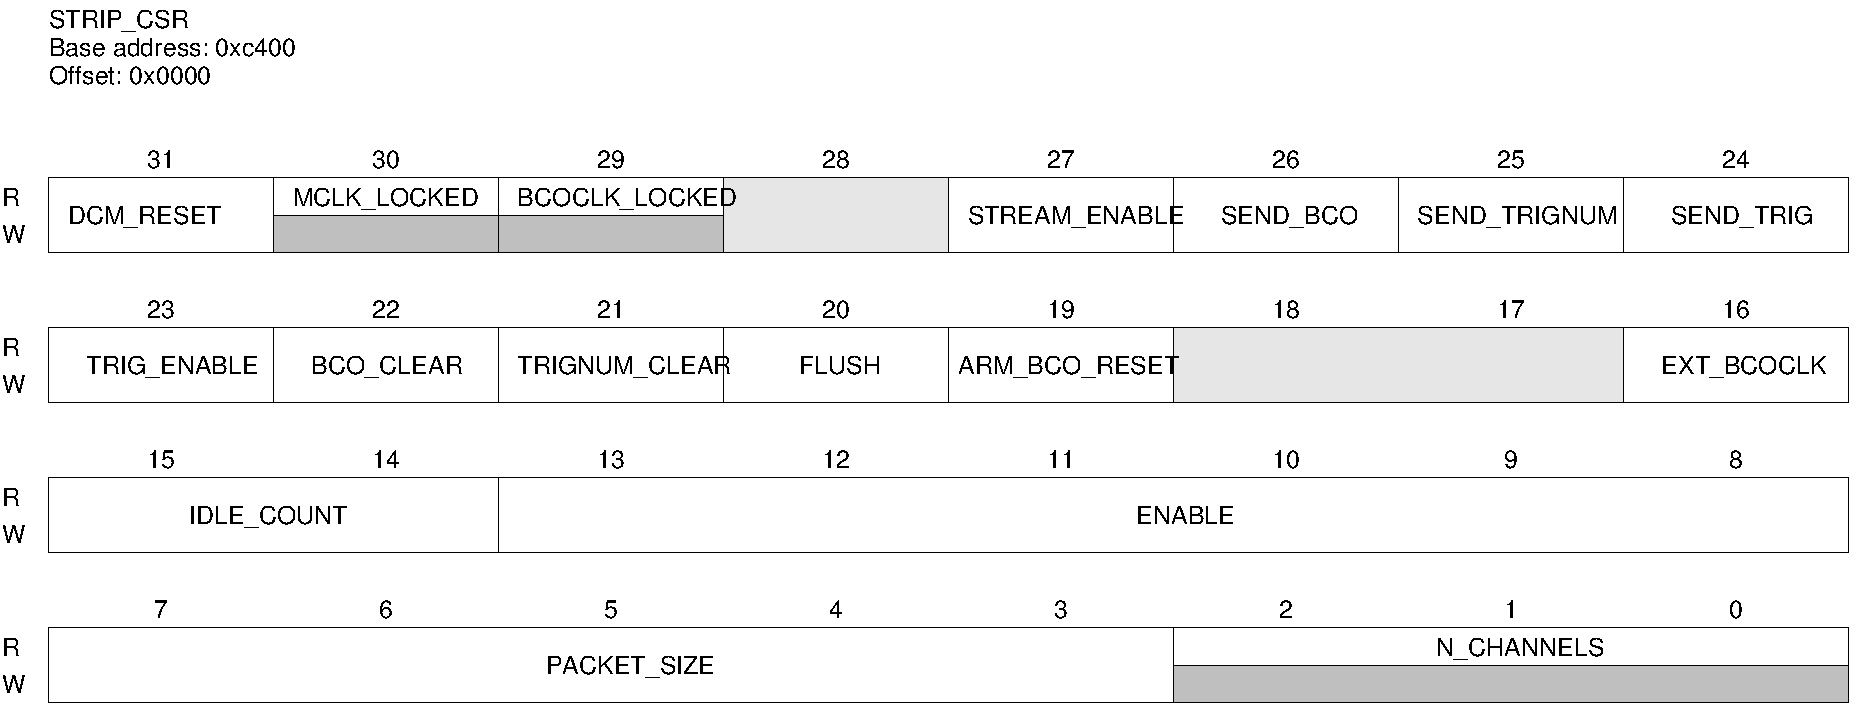
\includegraphics[width=16cm]{strip_csr.pdf}}

\begin{table}
\begin{center}
\small
\begin{tabular}{|c|c|c|l|} \hline
bits & name & access & description \\ \hline\hline
31 & DCM\_RESET & w/w & Assert RESET signal to the clock generator module \\
30 & BCO\_LOCKED & r & BCO frequency locked \\
29 & MCLKA\_LOCKED & r & MCLK\_A frequency locked \\
28 & MCLKB\_LOCKED & r & MCLK\_B frequency locked \\
27 & BCO\_CLEAR & r/w & resets BCO counter to zero \\
26 & BCO\_ENABLE & r/w & enables BCO counter increment \\
25 & STREAM\_ENABLE & r/w & enables streaming hit data over Ethernet \\
24 & FLUSH & r/w & flushes buffered streaming hit data to network \\
23 & SEND\_BCO & r/w & Include BCO number in hit data stream \\
22--16 & unused & & \\
15--11 & BCO\_DIVISOR & r/w & 100 MHz clock divisor for BCO clock \\
10--8 & IDLE\_COUNT & r/w & Time to wait before dumping idle packet \\
7--3 & PACKET\_SIZE & r/w & Number of 32-bit hit words per packet \\
2--0 & N\_CHANNELS & r & Number of channels defined in firmware \\ \hline
\end{tabular}
\end{center}
\caption{\label{tab-stripcsr}STRIP\_CSR - address 0xc4000000.}
\end{table}

\clearpage
\subsubsection{Strip reset register}
Reset signals are asserted by setting the appropriate bits in the
STRIP\_RESET register.  These cause the specified reset signal to be
asserted for a fixed number of BCO clock cycles (currently 7), and
are self clearing.  While the reset signals are asserted, their status
is reflected by reading the appropriate bits in the register.  The
CHANNEL\_MASK bits select the channels to whcih the reset signals are
simultaneously sent.  Note that asserting CHIP\_RESET does not automatically
assert LINK\_RESET.  Normally CHIP\_RESET and LINK\_RESET should be
asserted simultaneously to cause the link to be resynchronized after the
chip comes out of reset.

% \centerline{\epsfxsize=16cm\epsffile{strip_reset.eps}}
\centerline{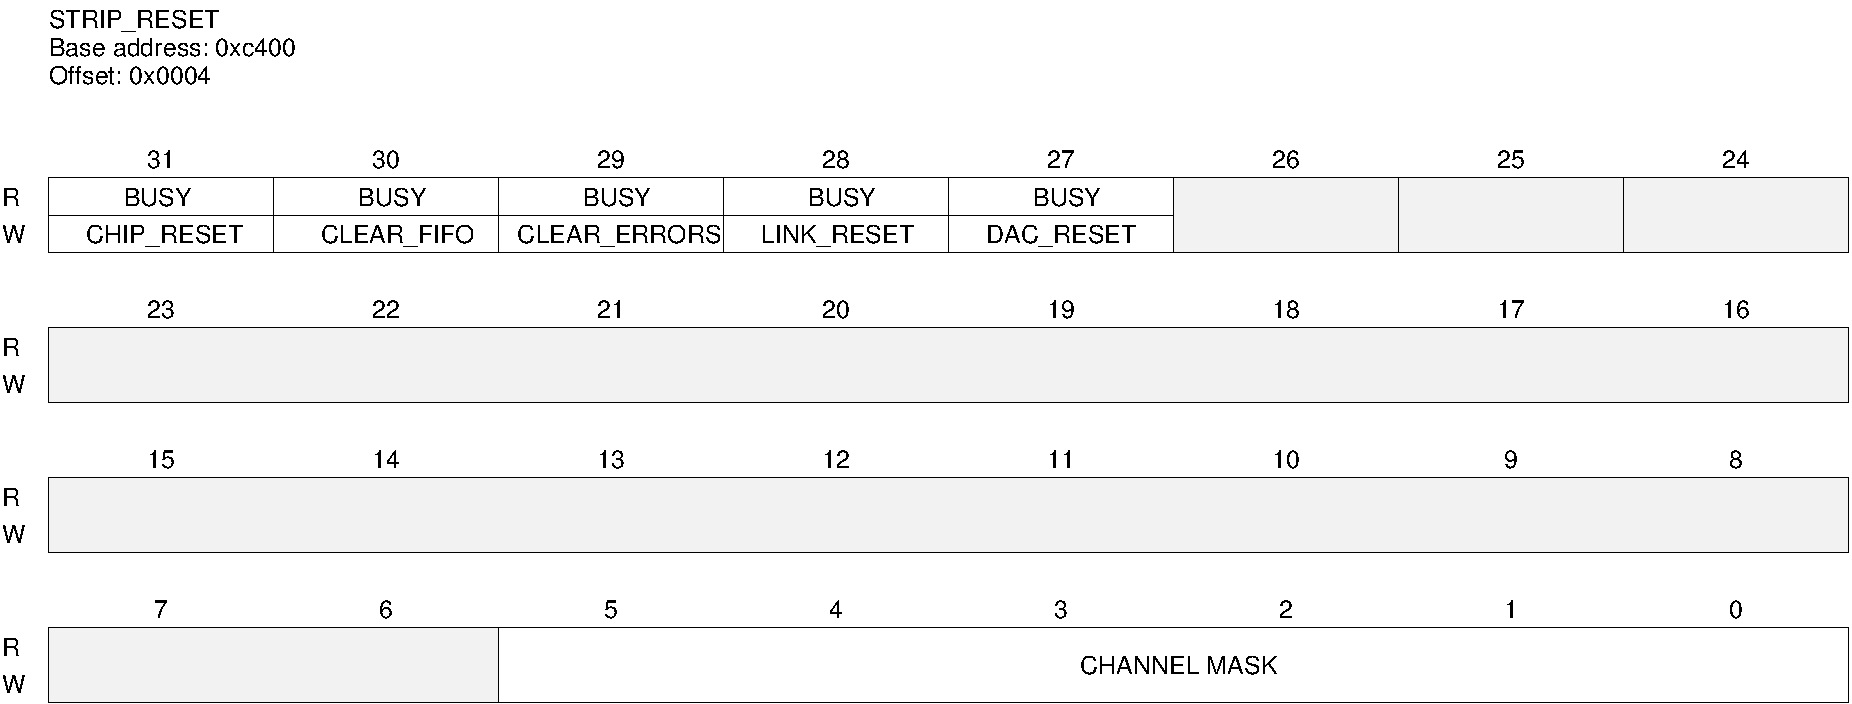
\includegraphics[width=16cm]{strip_reset.pdf}}

\begin{table}
\begin{center}
\small
\begin{tabular}{|c|c|c|l|} \hline
bits & name & access & description \\ \hline\hline
31 & CHIP\_RESET & w & Assert RESET signal on selected channels \\
   &             & r & Indicates that RESET signal is asserted \\ \hline
30 & CLEAR\_FIFO & w & Clears link spy FIFO's \\
   &             & r & Istatus of FIFO clear signal \\ \hline
29 & CLEAR\_ERRORS & w & Clears link error counters \\
   &               & r & Status of link error counter reset signal \\ \hline
28 & LINK\_RESET & w & Causes the selected links to realign and synchronize \\
   &             & r & Status of link reset signal \\ \hline
27 & DAC\_RESET & w & Asserts the reset* signal to the DAC's (not masked)\\
   &            & r & Status of the DAC reset signal \\ \hline
7..0 & CHANNEL\_MASK & r/w & Reset signals are sent to all channels with bits \\
     &               &     & set in the CHANNEL\_MASK field \\ \hline
\end{tabular}
\end{center}
\caption{\label{tab-stripreset}STRIP\_RESET - address 0xc4000004.}
\end{table}

\clearpage
\subsubsection{Slow controls command register}
There are two modes of operation for the STRIP\_SC register which depend on
the value of the RAW bit (bit 30).  When RAW=0, the different bit fields
specify the slow controls register operation to be performed.  When
RAW=1, bits contained in the STRIP\_SCI[0..3] registers are shifted out
without interpretation.  The slow controls bits are shifted on the
SHIFT/SCIN lines of all channels selected by the CHANNEL\_MASK field and
the SCOUT data received from the single channel selected by the READ\_CHANNEL
is stored in the STRIP\_SCO[0..3] registers.  When RAW=0, the LENGTH field
encodes the number of data bits to be sent or received according to
Table~\ref{tab-sclen}.
\begin{table}
\begin{center}
\small
\begin{tabular}{|c|c|} \hline 
value & number of bits \\ \hline
0 & 0 \\
1 & 1 \\
2 & 2 \\
3 & 8 \\
4 & 128 \\ \hline
\end{tabular}
\end{center}
\caption{\label{tab-sclen}Encoded length parameter values in
the STRIP\_SC register.}
\end{table}

% \centerline{\epsfxsize=16cm\epsffile{strip_sc.eps}}
\centerline{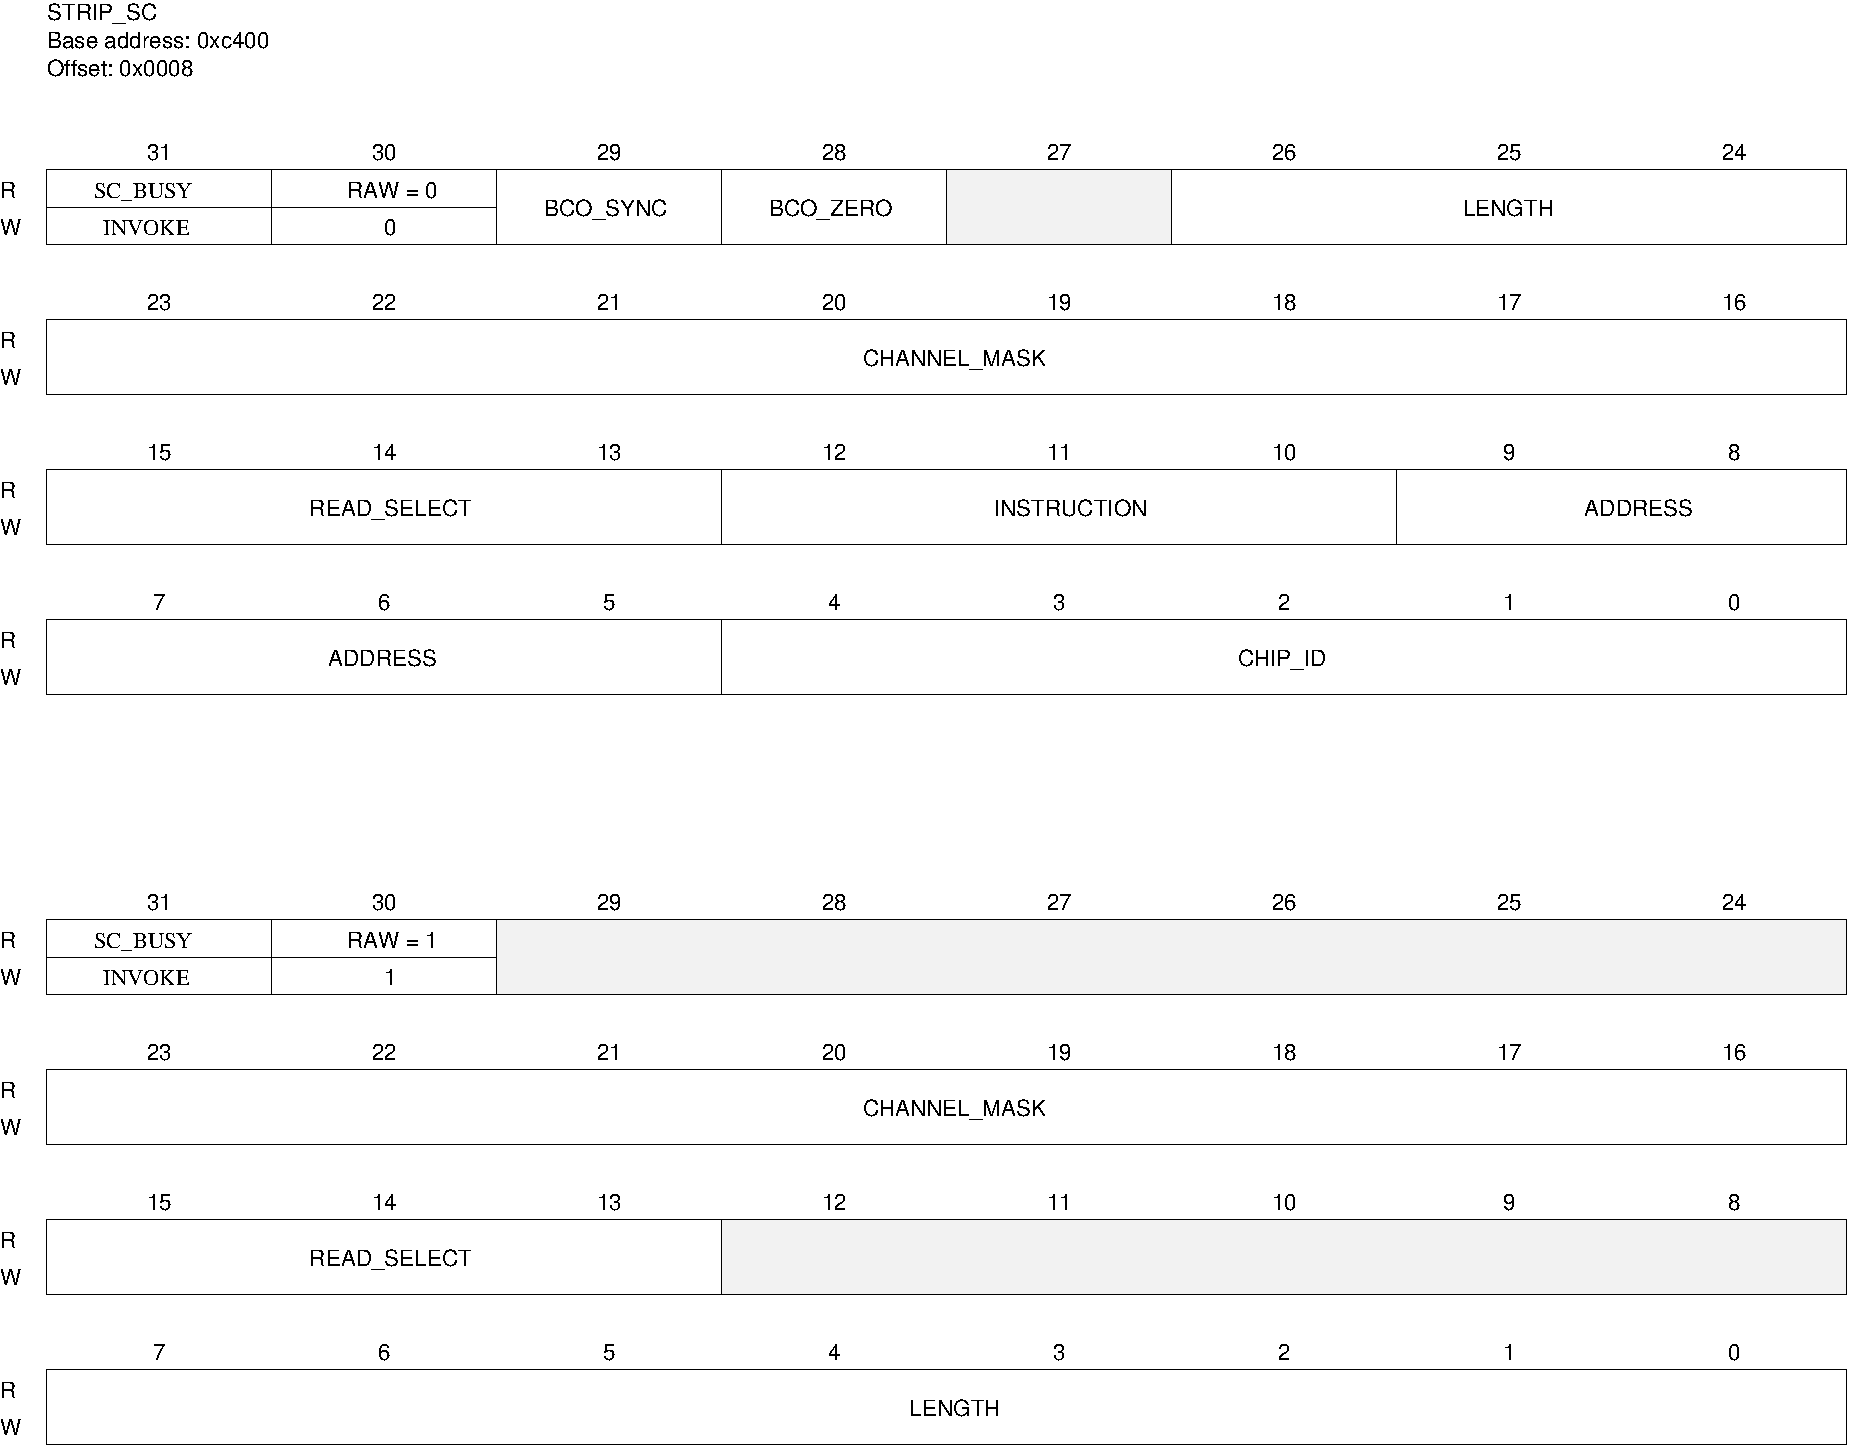
\includegraphics[width=16cm]{strip_sc.pdf}}
\begin{table}
\begin{center}
\small
\begin{tabular}{|c|l|c|l|} \hline
bits & name & access & description \\ \hline\hline
31 & SC\_BUSY & r & Set while a slow controls transaction is in progress \\ \hline
   & INVOKE      & w & Initiate the slow controls transaction \\ \hline
30 & RAW & r/w & Set when raw data is being shifted out \\ \hline
29 & BCO\_SYNC  & r/w & Synchronize rising edge of SHIFT with BCO zero  \\ \hline
28 & BCO\_ZERO  & r/w & Synchronize falling edge of SHIFT with BCO zero  \\ \hline
26-24 & LENGTH & r/w & Encodes the number of bits to send \\ \hline
23-16 & CHANNEL\_MASK & r/w & Set bits enable the channels to receive SCIN \\ \hline
15-13 & READ\_SELECT & r/w & Select channel from which to read SCOUT \\ \hline
12-10 & INSTRUCTION & r/w & Slow-controls instruction \\ \hline
9-5 & ADDRESS & r/w & Slow-controls register address \\ \hline
4-0 & CHIP\_ID & r/w & Target chip ID \\ \hline
\end{tabular}
\end{center}
\caption{\label{tab-stripsc}STRIP\_SC - address 0xc4000008.}
\end{table}

When the BCO\_SYNC and BCO\_ZERO bits are not set, SHIFT is asserted
on the next falling edge of BCOCLK and is deasserted on the falling edge
of BCOCLK after all bits have been shifted.

When BCO\_SYNC is set, the
transaction is dealyed until the internal BCO counter has a value of 240
and SHIFT is deasserted on the first rising edge of BCOCLK after all bits
have been shifted.  This allows the AqBCO command to be synchronized in
such a way that it will latch the bunch counters internal to the chips
when they equal zero and cause the AqBCO status bit to be asserted.  If
the BCO counter internal to the chips is not equal to zero, then the AqBCO
status bit will be cleared.  Figure~\ref{fig-aqbco} shows the timing
when BCO\_SYNC is set.
\begin{figure}
%%  \centerline{\epsfxsize=10cm\epsffile{scr_scope.eps}}
  \centerline{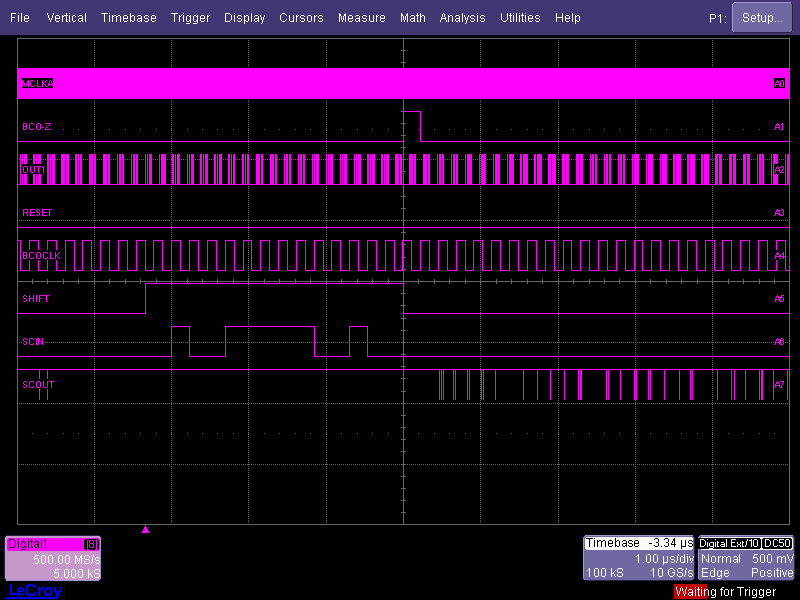
\includegraphics[width=12.8cm,height=9.6cm]{aqbco_scope.png}}
  \caption{\label{fig-aqbco}Example of the (AqBCO,Set) command when BCO\_SYNC=1.}
\end{figure}

When BCO\_ZERO is set, SHIFT will be held high until the falling edge
of BCOCLK one cycle before the BCO=0.  In this way, the SCR command can be
timed so as to synchronize the BCO counters internal to the chips with the
counter implemented in the STIB firmware.  After this synchronization has
been performed, AQBCO commands sent with the BCO\_SYNC set will always latch
BCO=0 into the AqBCO output register and set the AqBCO status bit, unless 
bunch counter synchronization has been lost.
\begin{figure}
%%  \centerline{\epsfxsize=10cm\epsffile{scr_scope.eps}}
  \centerline{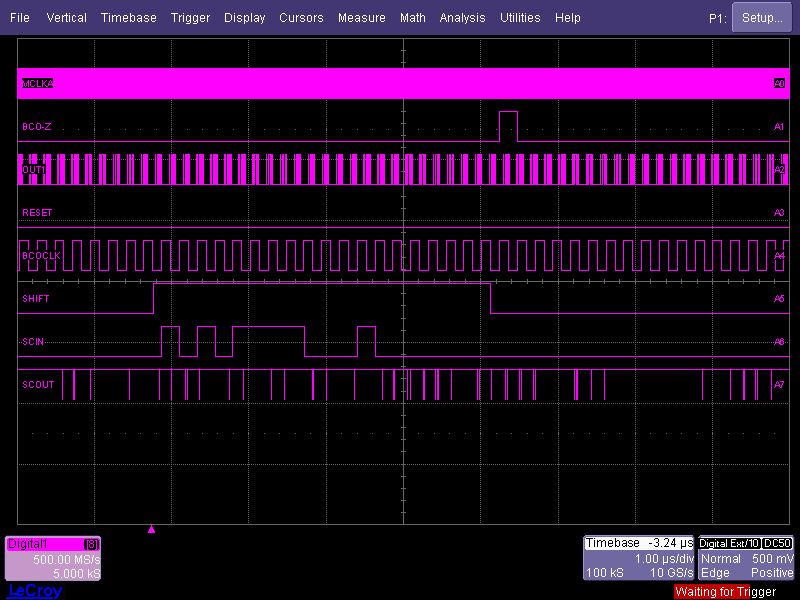
\includegraphics[width=12.8cm,height=9.6cm]{scr_scope.png}}
  \caption{\label{fig-scr}Example of the (SCR,Set) command when BCO\_ZERO=1.}
\end{figure}

\clearpage
\subsubsection{Link status register}

% \centerline{\epsfxsize=16cm\epsffile{strip_serdes_status.eps}}
\centerline{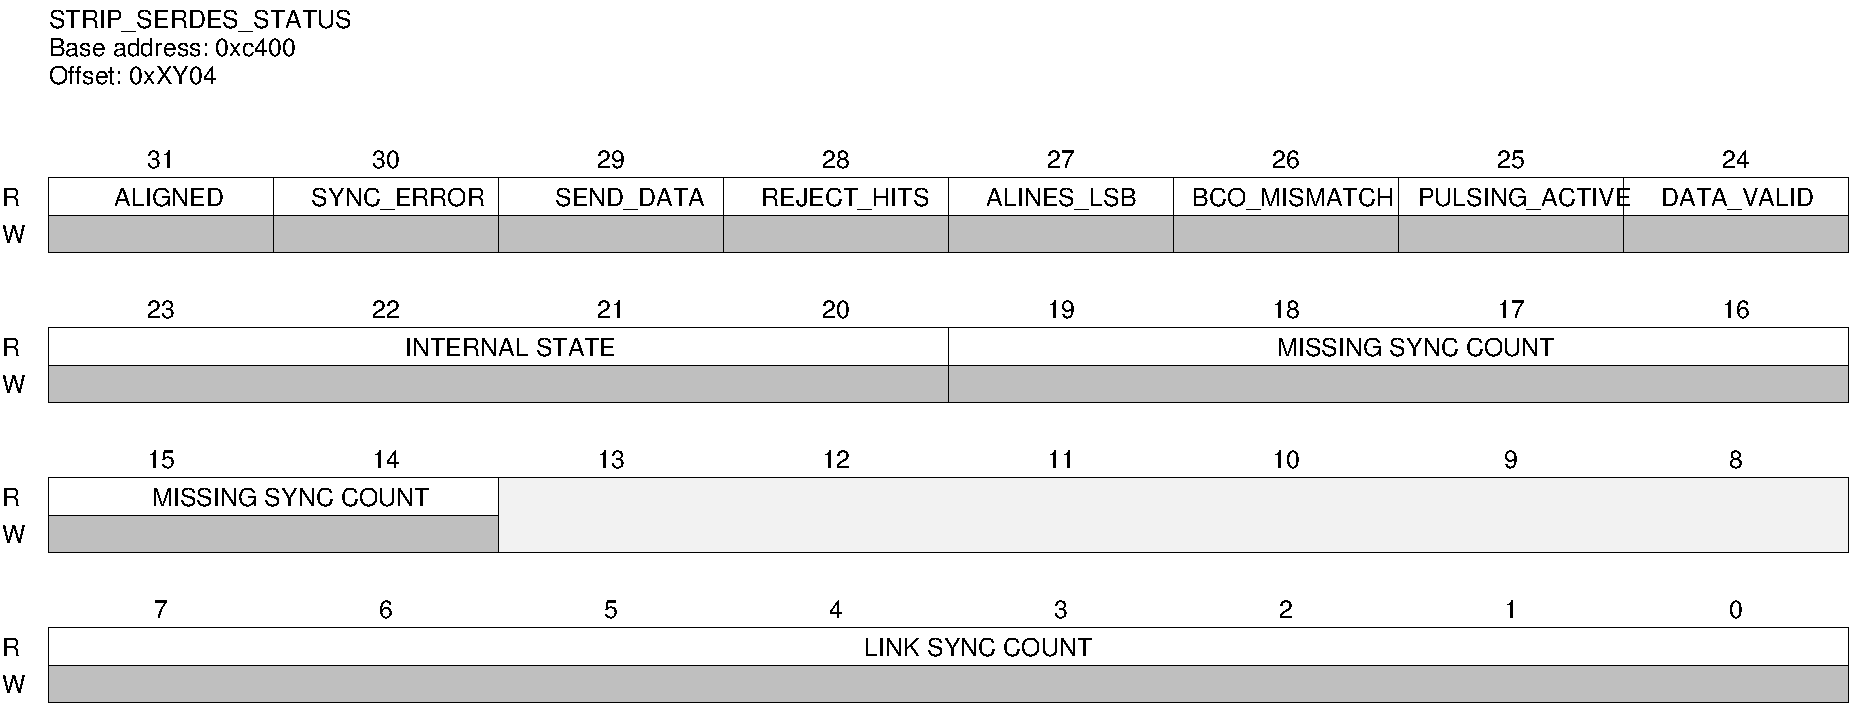
\includegraphics[width=16cm]{strip_serdes_status.pdf}}

\begin{table}
\begin{center}
\small
\begin{tabular}{|c|l|c|l|} \hline
bits & name & access & description \\ \hline\hline
31 & ALIGNED & r & Set when the sync word is successfully aligned \\ \hline
30 & SYNC\_ERROR & r & Set for one OUTCLK cycle when a single sync \\
   &             &   & error detected \\ \hline
29 & SEND\_DATA  & r & SendData - copied from sync word status bits \\ \hline
28 & REJECT\_HITS & r & RejectHits - copied from sync word status bits \\ \hline
27 & ALINES\_LSB & r & Alines LSB - copied from sync word status bits \\ \hline
26 & BCO\_MISMATCH & r & Acquire BCO = 1 if number $\ne$ 0 - copied \\
   &               &   & from sync word status bits \\ \hline
25 & PULSING\_ACTIVE & r & copied from sync word status bits \\ \hline
24 & DATA\_VALID & r & Valid data on FIFO input \\
23-20 & INTERNAL\_STATE & r & internal state of link serdes FSM \\ \hline
19-14 & MISSING\_SYNC\_COUNT & r & Number of consecutive data words received with \\
      &                      &   & no intervening sync words \\ \hline
13-8 & DELAY\_TAP\_COUNT & r & Tap count applied to IDELAY \\ \hline
7-0  & LINK\_SYNC\_COUNT & r & Number of OUTCLK cycles needed to synchronize \\
     &                   &   & link \\ \hline
\end{tabular}
\end{center}
\caption{\label{tab-serdesstatus}STRIP\_SERDES\_STATUS - address 0xc400$xy$04.}
\end{table}

\clearpage
\subsubsection{Serial data analyais}
The {\tt stripana} module accumulates statistics about hit data retrieved
by spying on the input to the channel FIFO.  Only data with
STRIP\_NUMBER and SET\_NUMBER matching the fields in the
STRIP\_ANALYSIS\_CSR are analyzed.  Mapping between set/strip number
and strip channel number is provided in Tables~\ref{tab-strip}
and~\ref{tab-set}.

\begin{table}
\begin{center}
\begin{minipage}{4cm} {
  \begin{tabular}{|c|c|} \hline
    Strip No. & Code \\ \hline
0 & 0101 \\
1 & 0111 \\
2 & 0110 \\
3 & 1110 \\ \hline
  \end{tabular}
}
\end{minipage}
\begin{minipage}{4cm} {
  \begin{tabular}{|c|c|} \hline
    Strip No. & Code \\ \hline
4 & 1010 \\
5 & 1011 \\
6 & 1001 \\
7 & 1101 \\ \hline
  \end{tabular}
}
\end{minipage}
\end{center}
\caption{\label{tab-strip}Strip number encoding.}
\end{table}

\begin{table}
\begin{center}
\begin{minipage}{4cm} {
  \begin{tabular}{|c|c|} \hline
    Set No. & Code \\ \hline
0 & 01010 \\
1 & 01011 \\
2 & 01111 \\
3 & 01110 \\
4 & 01100 \\
5 & 01101 \\
6 & 11101 \\
7 & 11100 \\ \hline
  \end{tabular}
}
\end{minipage}
\begin{minipage}{4cm} {
  \begin{tabular}{|c|c|} \hline
    Set No. & Code \\ \hline
8  & 10100 \\
9  & 10101 \\
10 & 10111 \\
11 & 10110 \\
12 & 10010 \\
13 & 10011 \\
14 & 11011 \\
15 & 11010 \\ \hline
  \end{tabular}
}
\end{minipage}
\end{center}
\caption{\label{tab-set}Set number encoding.}
\end{table}

There are six 32-bit counters that record the number of BCO clock cycles
and the number of hits received from each chip.  When CLEAR is asserted,
all counters are reset to zero.  When CLEAR is deasserted,
statistics are accumulated until the BCO counter reaches a terminal count
value specified by the TERM\_COUNT\_BIT field.  For example, setting
TERM\_COUNT\_BIT = 26 terminates the accumulation of statistics when
the BCO count reaches 0x04000000.  During and after accumulation, the
counters can be read via the STRIP\_ANALYSIS\_BCO\_COUNTER and 
STRIP\_ANALYSIS\_HIT$y$\_COUNTER registers where $y=1..5$.

% \centerline{\epsfxsize=16cm\epsffile{strip_ana.eps}}
\centerline{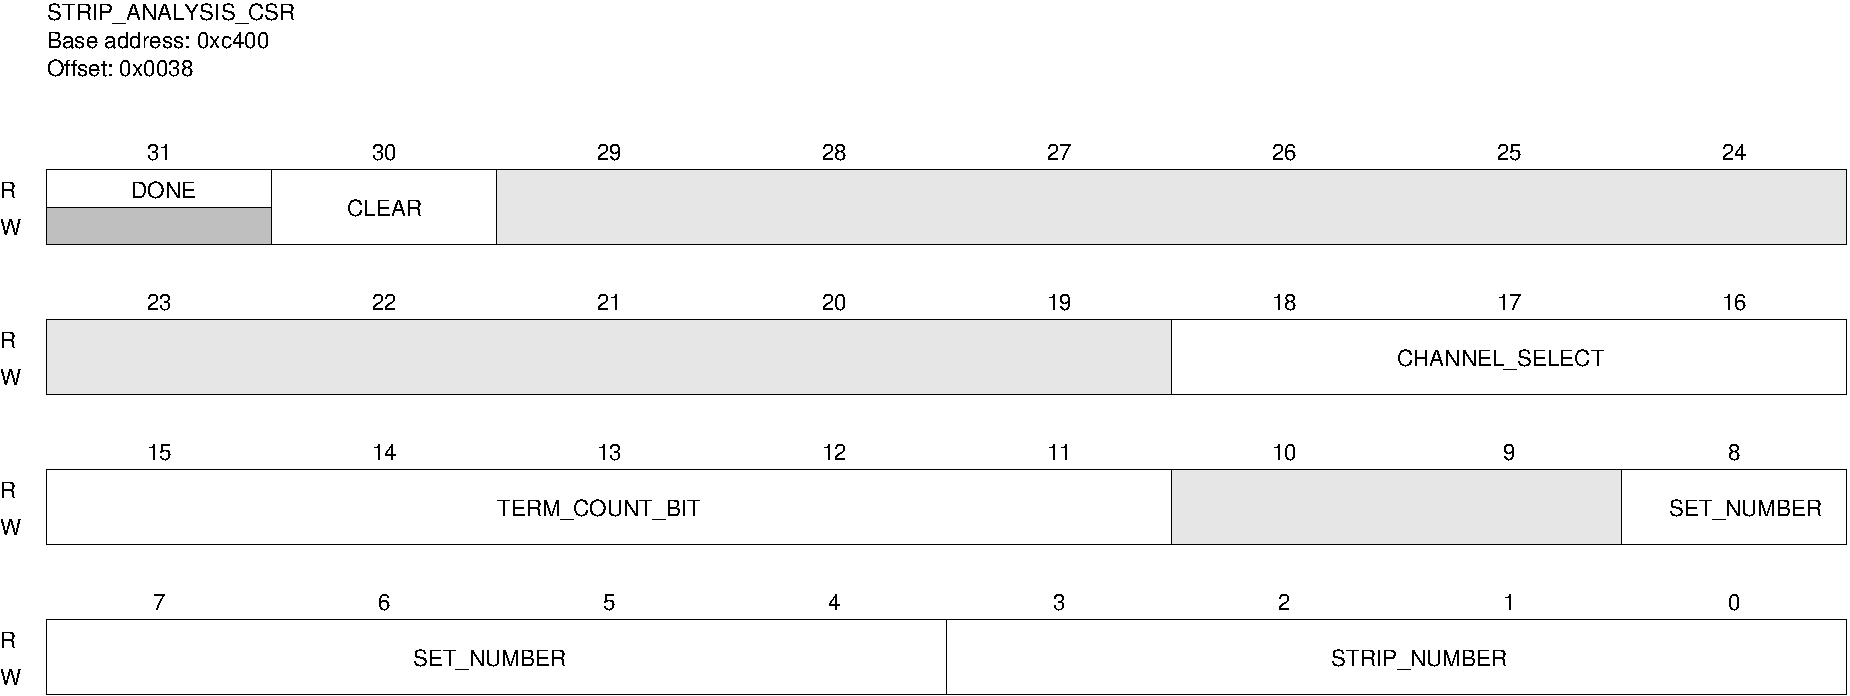
\includegraphics[width=16cm]{strip_ana.pdf}}

\begin{table}
\begin{center}
\small
\begin{tabular}{|c|l|c|l|} \hline
bits & name & access & description \\ \hline\hline
31 & DONE & r & Indicates that the terminal BCO count has been reached \\ \hline
30 & CLEAR & r/w & Resets all counters - not self clearing \\ \hline
18..16 & CHANNEL\_SELECT & r/w & Selects strip sensor channel for analysis \\ \hline
15..11 & TERM\_COUNT\_BIT & r/w & $\log_2$ of BCO count at which to stop analysis \\ \hline
8..4 & SET\_NUMBER & r/w & Set number to match in data stram \\ \hline
3..0 & STRIP\_NUMBER & r/w & Strip number to match in data stram \\ \hline
\end{tabular}
\end{center}
\caption{\label{tab-stripanacsr}STRIP\_ANALYSIS\_CSR - address 0xc4000038.}
\end{table}

\subsection{Streamed data interface}
Hit data is collected from all channels into a single fifo and sent
as UDP packets over the Ethernet link.  The destination address is
stored in the STREAMPKT\_DADDR (0xc10000a4) register and the source
and destination ports are stored in the STREAMPKT\_PORTS (0xc10000a8)
register.  Data will be written to a FIFO when bit 25 in the STRIP\_CSR
register is set and will be transmitted over Ethernet when the number
of words written equals the number encoded in the PACKET\_SIZE field of
the STRIP\_CSR register.  The number of 32 bit words per packet is
given by
\begin{equation}
  n = 16 \times (\mbox{PACKET\_SIZE} + 1)
\end{equation}
or $n=350$ when PACKET\_SIZE = 0x1f.  Except for this case, packet
sizes must be smaller than the maximum transfer unit of approximately
1500 bytes on typical netowrks.  The choice of packet size is a tradeoff
between latency and the effective use of the network bandwidth for data
rather than frame/packet header information.
If hit generation has been disabled, the data that remains in the FIFO can
be flushed by setting the FLUSH bit in the STRIP\_CSR register.

Streamed data consist of 32-bit words in which low bits to define
their data type.  Hit data from the FSSR2 chips has the lowest bit
set to 1 (this is a sync bit), so any data word with the lowest order bit
set to zero indicates some other data type.  In particular, a status word
is indicated by the lowest 4-bits set to "1000", and hit data from a
detector that uses another type of readout chip could be indicated by other
bit patterns, provided they don't conflict with these ones.
Table~\ref{tab-datatype} lists the bit patterns that are currently defined
or envisioned.
\begin{table}
\begin{center}
\begin{tabular}{|c|c|c|}\hline
pattern & data type & figure number \\ \hline\hline
xxx1 & FSSR2 hit data & \ref{fig-fssr2data} \\
xx10 & PSI46 hit data &  -- \\
1000 & STIB status/data & \ref{fig-stibstat} \\ \hline
\end{tabular}
\caption{\label{tab-datatype}Data types indicated by the low 4-bits in the
32-bit streamed data words.}
\end{center}
\end{table}

Status words have the low 4-bits of the streamed data word set to "1000", 
with bits 7..4 specifying the type of status data provided in the upper
24-bits.  Figure~\ref{fig-stibstat} shows the format of the status words
that will be sent.
\begin{figure}
  \centerline{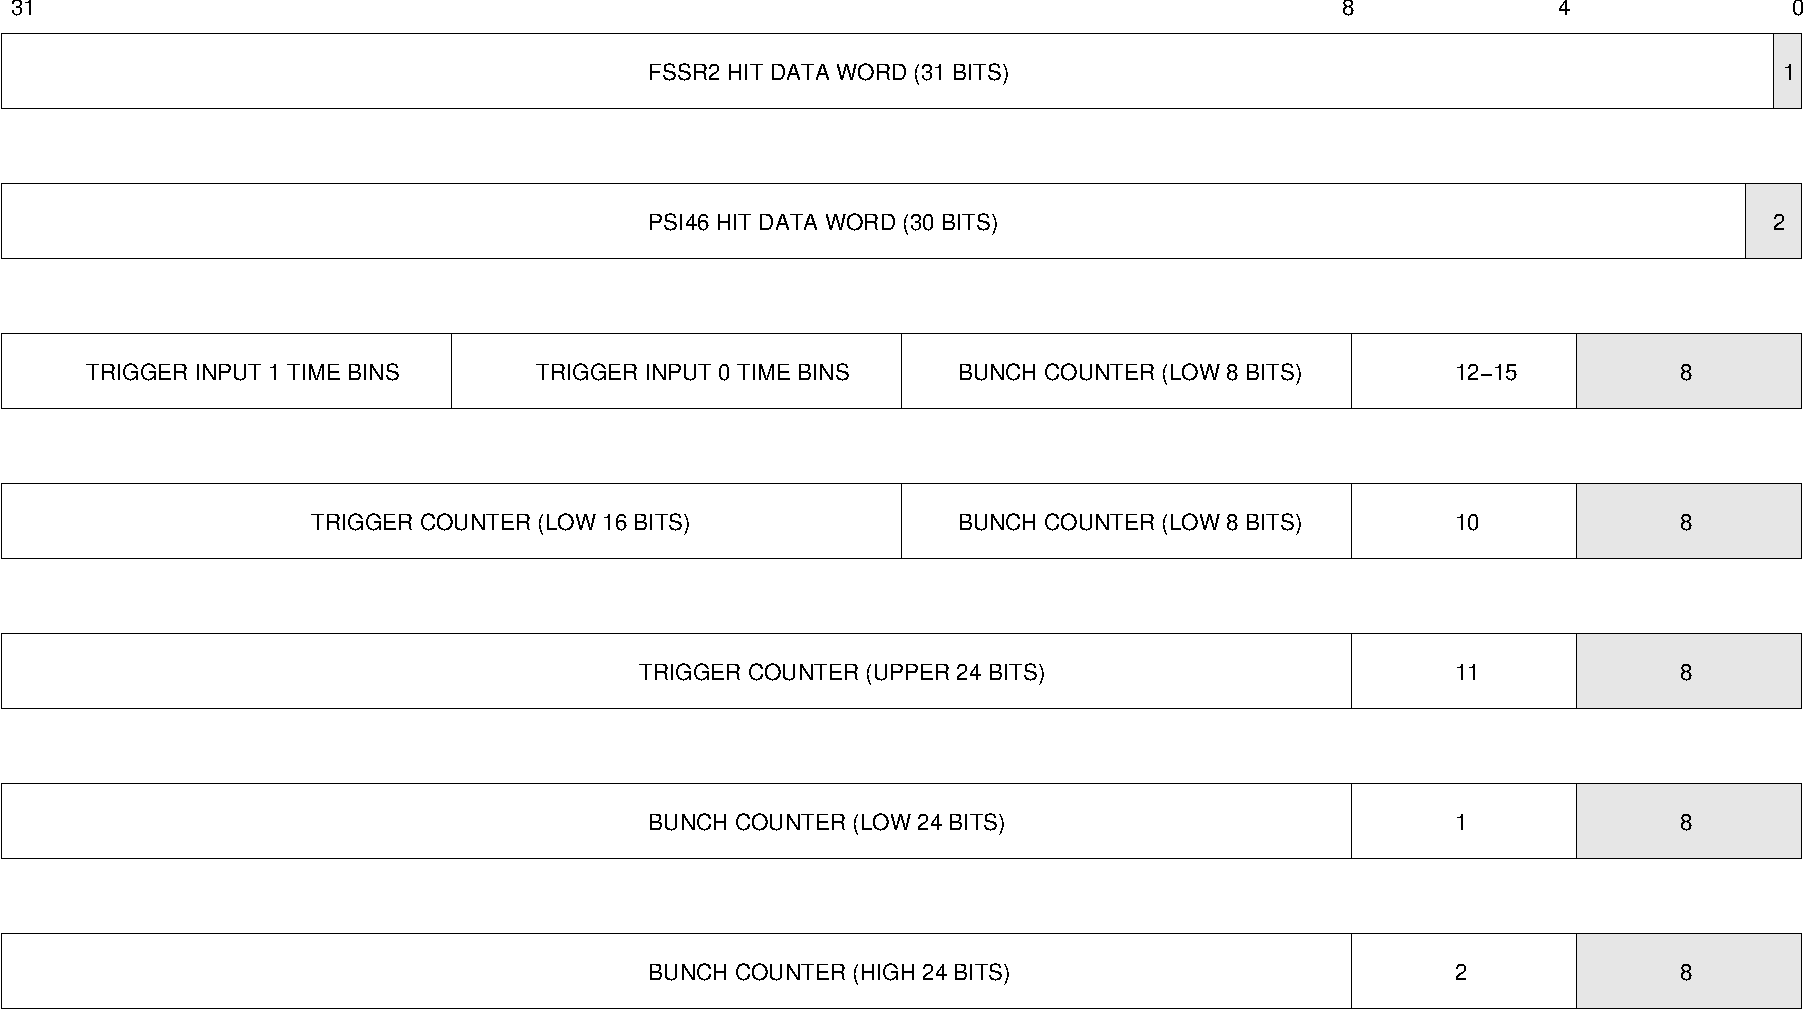
\includegraphics[width=15.5cm]{stibstat.pdf}}
  \caption{\label{fig-stibstat}Format of the streamed STIB status/data words.}
\end{figure}

\subsubsection{FSSR2 data}
Figure~\ref{fig-fssr2data} defines the data word for FSSR2 strip hits.
\begin{figure}
  \centerline{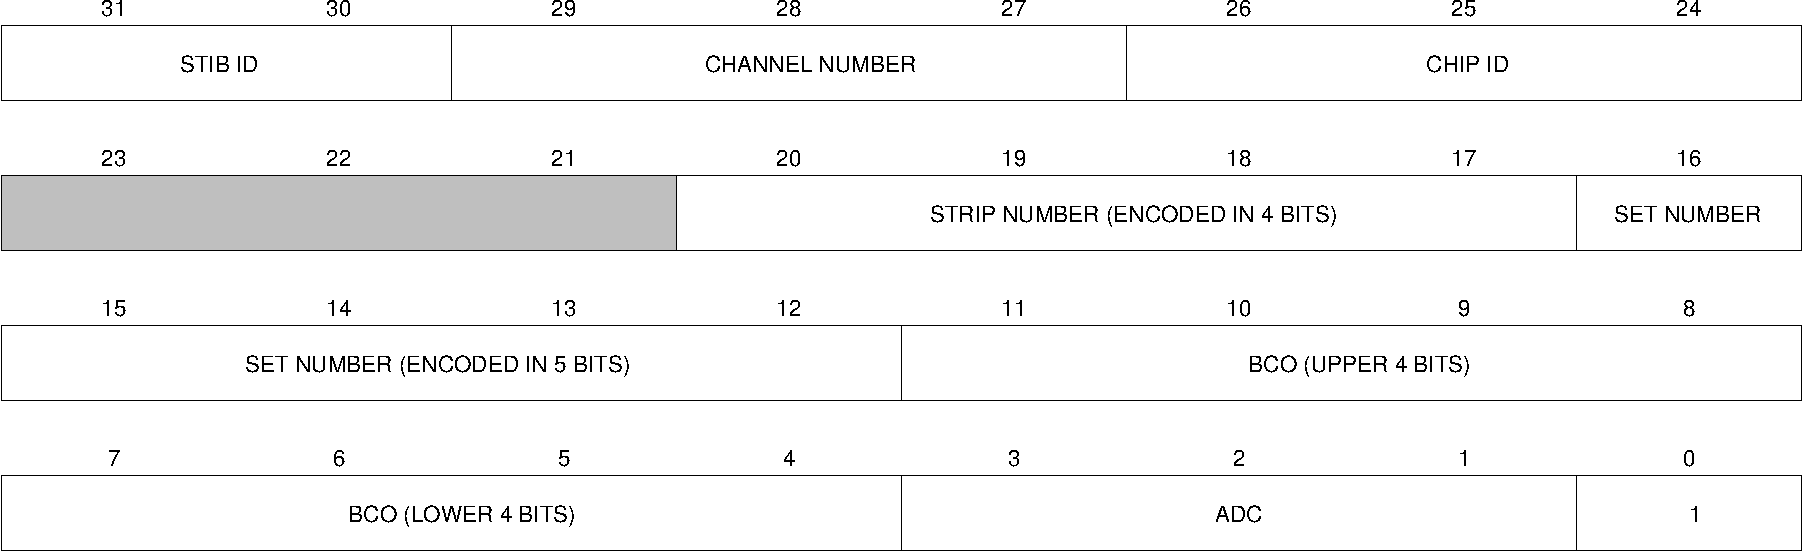
\includegraphics[width=15.5cm]{fssr2data.pdf}}
  \caption{\label{fig-fssr2data}Format of the streamed FSSR2 hit data word.}
\end{figure}

\subsubsection{PSI46 data}
Data words from pixel hits read out using the PSI46 ROC may be packed into
30 bits in a format to be defined elsewhere.

\subsubsection{STIB scintillator data (proposed)}
The scintillator data word can pack two input channels into a 16-bit word.
Each 8-bit channel data corresponds to a 2-bit channel number and 6 bits
that mask the fine time bins in which the singnal was present.  Alternatively,
we could pack the data like the proposed hit-or data word (below) which
just stores the time of the first hit.

\subsubsection{STIB hit-or data (proposed)}
The hit-or outputs from 2 channels can be packed into a 16-bit word.
Each 8-bit channel data corresponds to a 3-bit channel number and a 5-bit
word that measures the fine-binned time at which the hit arrived (assuming
this is meaningful).

\subsubsection{Bunch counter data}
Bunch counter words are sent when bit 23 of the STRIP\_CSR word is set.
Bunch counter information is only transmitted immediately before a valid hit
if no bunch counter words have been previously been sent within
the past 256 BCO clock cycles.  In this way, the all information needed to
determine the full 48-bit BCO counter is available as soon as the hit data
words are received.  For low rates, 2/3 of the data bandwidth is used by
the BCO counter words, but this fraction is reduced to less than 1\% of the
data bandwidth at high rates.

\subsubsection{Trigger data (proposed)}
Trigger data is sent using two 32-bit status words.  The first word
contains the 8-bit BCO number of the triggered event and the low 16-bits
of the trigger counter, which is incremented for each triggered event.
The second trigger data word contains the upper 8-bits of the 24-bit trigger
counter and four 4-bit trigger masks indicating the status of the trigger
inputs on the previous, current and subsequent two BCO clocks.  The four
trigger input bits may be defined according to Table~\ref{tab-trigprim}.
\begin{table}
  \begin{center}
    \begin{tabular}{|c|c|}\hline
bit & trigger input \\ \hline
0 & prescale (0 will skip readout) \\
1 & external trigger input (ie, scintillator) \\
2 & hit-or trigger input \\
3 & slave trigger input \\ \hline
\end{tabular}
  \end{center}
  \caption{\label{tab-trigprim}Bits defining trigger primitive inputs.}
\end{table}
The prescale bit is set on BCO cycles for which readout is intended and is
set by the master STIB.  The external trigger input would be set by the
gated scintillator trigger logic, or by any other external digital signal.
The hit-or trigger input is derived from the pattern of hit-or signals
received from the FSSR2 hybrids.  The slave trigger input corresponds to
the logical OR of trigger signal received from slave STIB boards, which may
internally form their own trigger logic based on, for example, the FSSR2
hit-or signals.  The global trigger, which initiates readout, would then be
defined by a set of valid 4-bit patterns.  For example, to trigger on
non-prescaled BCO cycles, with scintillator trigger input and a hit-or
signal from at least one STIB board would require matching either "1011",
"0111" or "1111".

The internally generated hit-or trigger may be derived from the patterns
of hit-or signals received from individual FSSR2 hybrid channels.  A typical
scenario would be to require some minimal number of planes with simultaneous
hits on both X and Y channels.

\subsection{DAC interface}
There are four MAX5893 12-bit 500 MSPS DAC's on the STIB that are configured
by means of an SPI interface through the STRIP\_DAC\_SPI register.  The
bit fields in this register are shown in Figure~\ref{fig-dacspi}.
\begin{figure}
  \centerline{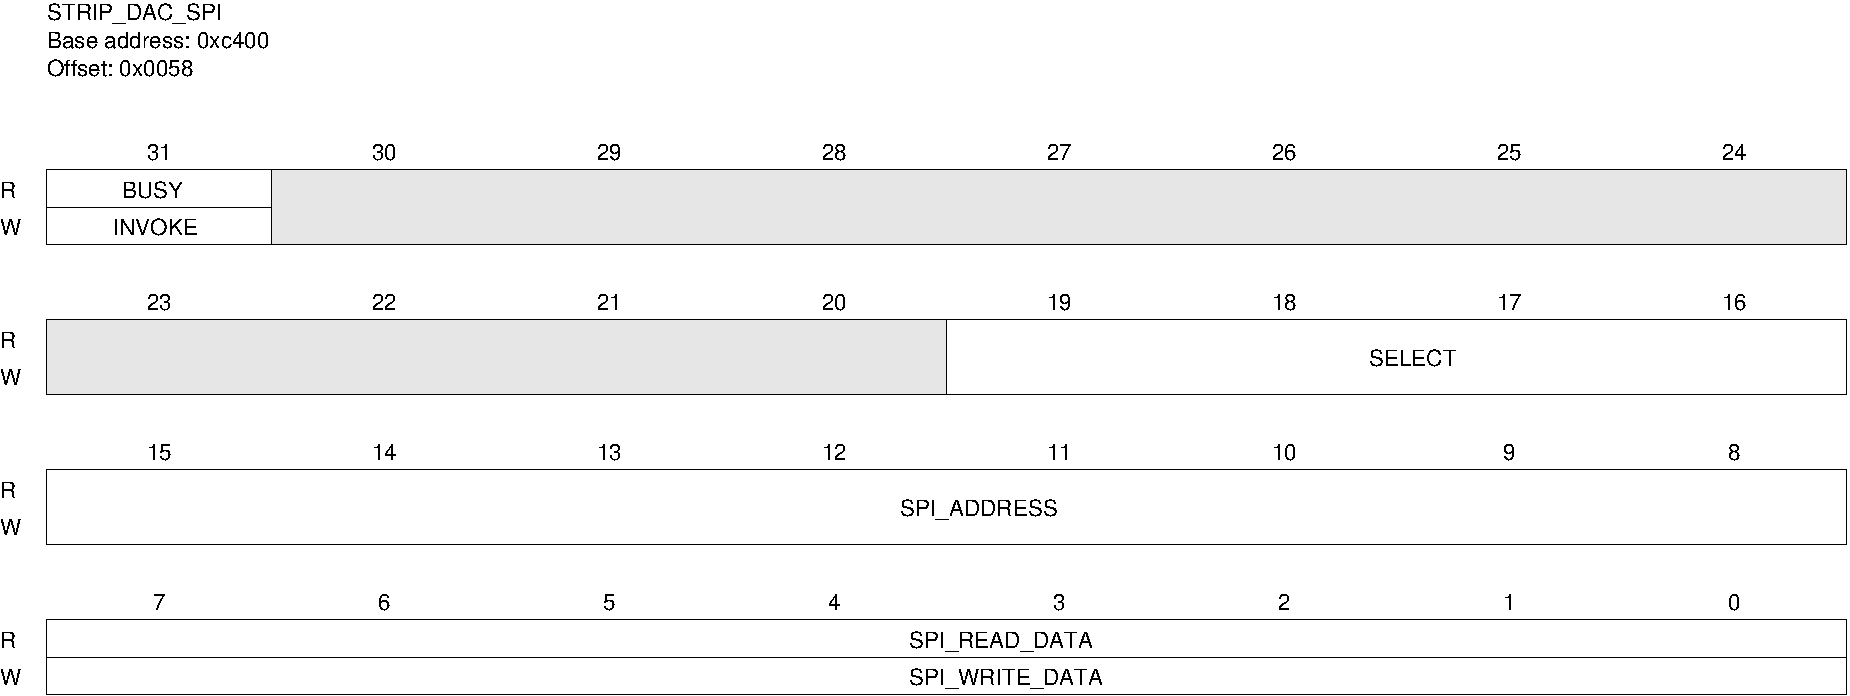
\includegraphics[width=16cm]{strip_dacspi.pdf}}
  \caption{\label{fig-dacspi}DAC SPI interface register.}
\end{figure}
Individual DAC's are addressed by the corresponding bits in the SELECT
field.  A write operation is requested when bit 16 is set to zero in which
case the data stored in the low 8-bits of the STRIP\_DAC\_SPI register is
stored in the addressed SPI register.  When bit 16 is '1', an SPI register
read is requested and the data from the addressed register is shifted in
and made available for reading as the low 8-bits of the STRIP\_DAC\_SPI
register.  Note that there is a one read-cycle latency before the data
appears.

The normal register configuration is to write 0 to register 0, 0x44 to register
1 and 0x40 to register 2.  The DAC can be disabled and put into a low-power
sleep state by writing 0x1c to register 0.

The STRIP\_DAC\_CSR register, shown in Figure~\ref{fig-daccsr},
controls the trigger conditions for pulse
generation.
\begin{figure}
  \centerline{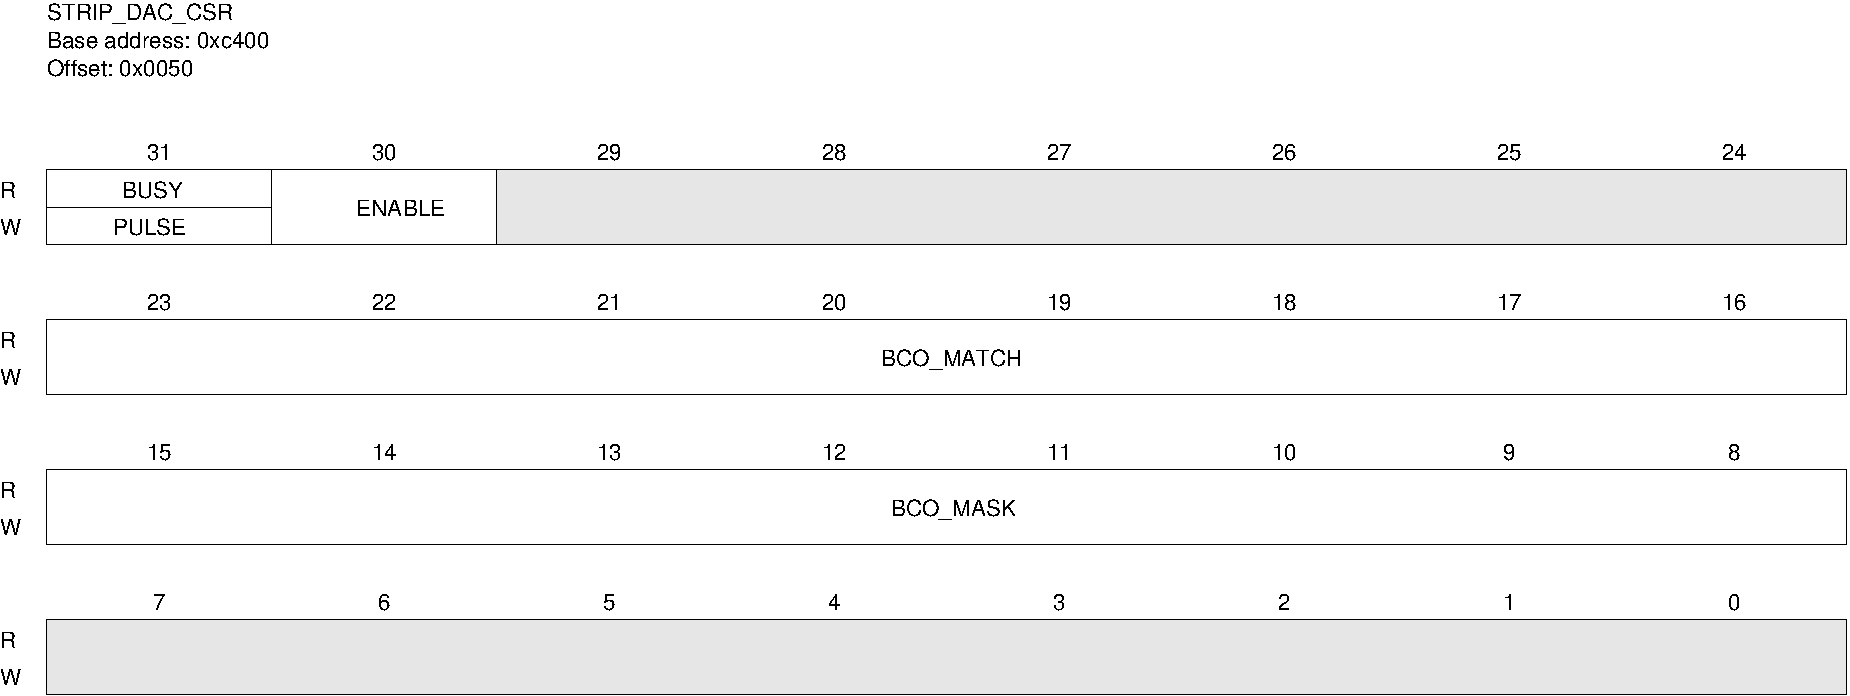
\includegraphics[width=16cm]{strip_daccsr.pdf}}
  \caption{\label{fig-daccsr}DAC command/status register.}
\end{figure}
Bits 8..15 define an 8-bit mask and bits 16..23 define an 8-bit
pattern that must match the bitwise AND of the low 8-bits of the BCO counter
and the mask in order to trigger a pulse when sampled on the falling edge
of BCOCLK.  A single pulse is generated by writing a '1' to bit 31, while
a continuous sequence of pulses is generated by writing a '1' to bit 30.
Reading from bit 31 indicates whether the DAC trigger interface is busy.

The amplitude and precise timing of the pulse is controlled by the
STRIP\_DAC\_VALUE register, shown in Figure~\ref{fig-dacval}.
\begin{figure}
  \centerline{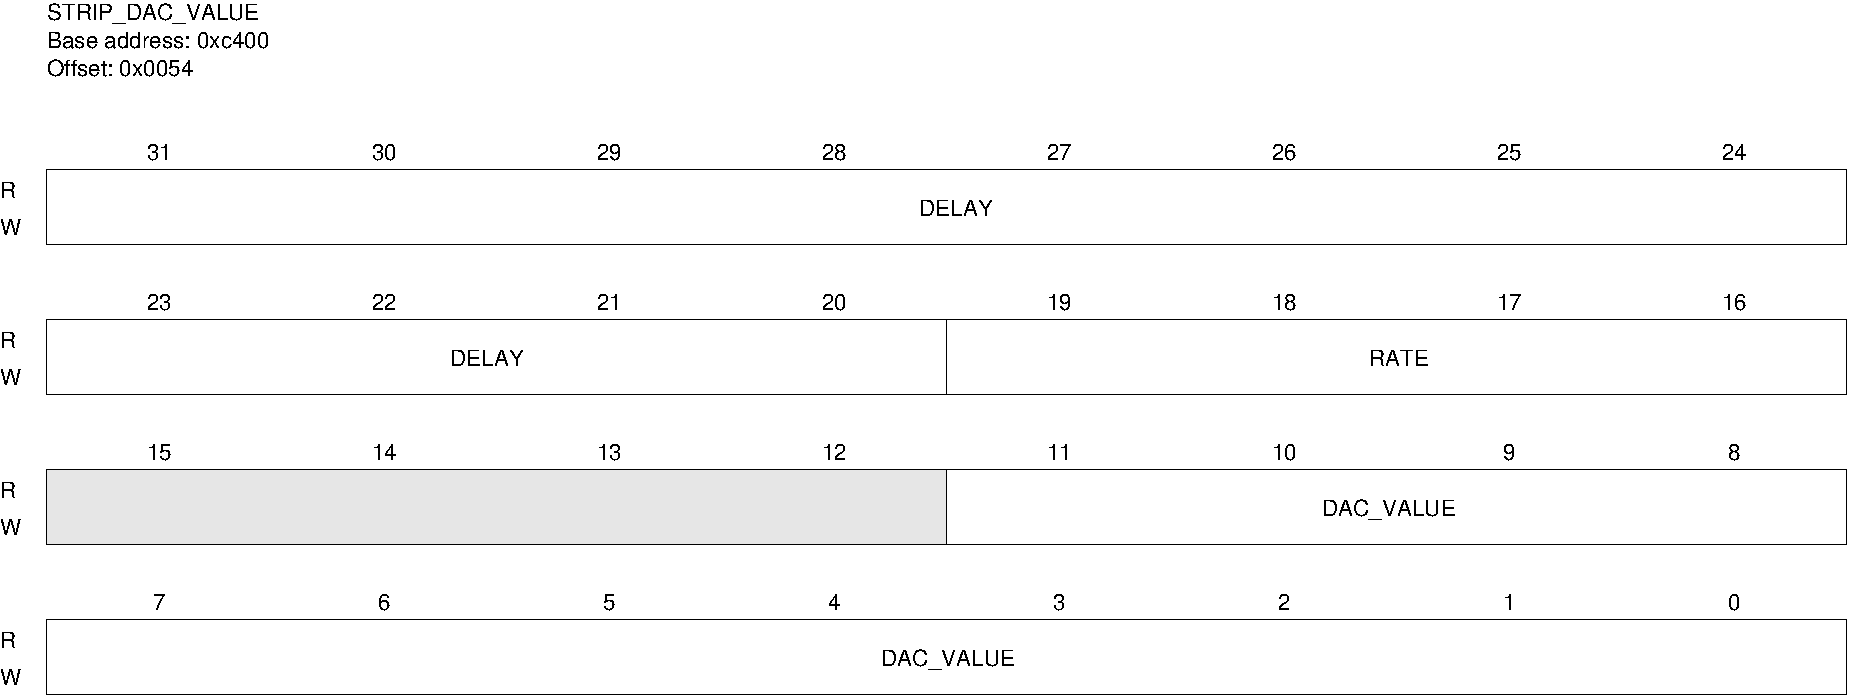
\includegraphics[width=16cm]{strip_dacval.pdf}}
  \caption{\label{fig-dacval}DAC pulse amplitude/delay control register.}
\end{figure}
Bits 20..31 define the terminal count for a
200 MHz counter that adjusts the timing after the matching BCO counter
before the pulse is generated.  This allows the pulse to be placed at any
point in the BCO sampling window.  Bits 16..19 define the rate at which
the pulse ramps back to baseline and bits 0..11 define the amplitude
of the voltage step generated by the DAC.  The FSSR2 chips respond to a
negative pulse, so this field requires a negative, signed, 2's compliment
number.  To protect the state machine from getting stuck, a rate of 1
is substituted in the case where bits 16..19 are all zero.

Figure~\ref{fig-dacscope} illustrates the timing of signals generated
when BCO\_MATCH = 0, DELAY = 0, VALUE = -512.  The pulse is generated
data is read out with BCO = 4 and data becomes available for writing to
the FIFO approximately 6 BCO clock cycles later.
\begin{figure}
  \centerline{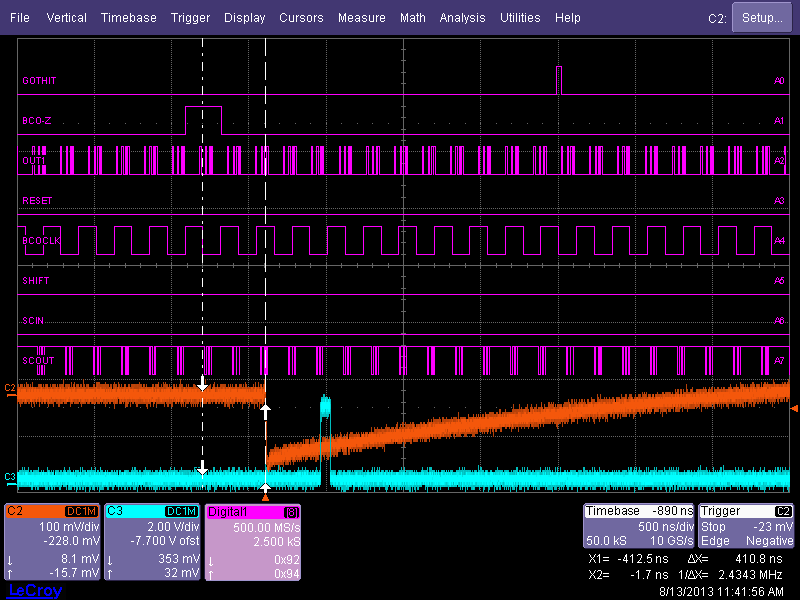
\includegraphics[width=12.8cm,height=9.6cm]{dac_scope.png}}
  \caption{\label{fig-dacscope}Example of DAC pulse timing.  Channel 2 is
the output of the DAC observed at the MMCX connector on the FSSR2 hybrid
board.  Channel 3 is the HITOR output of the FSSR2 chip in response to the
input pulse.  The observed delay between the trigger and the pulse output
is approximately 410 ns, mostly due to the data latency in the MAX5893 DAC.}
\end{figure}

\section{Command Line Interface}
The MicroBlaze core provides a command line interface that provides
extensive monitoring and debugging facilities.  While interaction with
the monitor is not required for normal operation, it provides valuable
feedback about many aspects of the internal state of the FPGA.
Most commands do nothing more than display memory contents using
context specific formats, or parse input arguments into bit
fields and write the result to specific memory mapped registers.
An interrupt handler processes incomming UDP packets, responding to
NTP and DHCP packets, and UDP packets that implement the bridge
between an external host on the network and the IOBUS address space.

\subsection{Low-level commands}
The low-level commands do not pertain to specific hardware
modules or address space.

\subsubsection{\tt led [on|off]}
Sets or clears a bit in the CAPTAN\_CSR register to turn on or off a
diagnostic LED.

\subsubsection{\tt peek \{address\}}
Displays the contents of the specified 32-bit memory address.

\subsubsection{\tt poke \{address\} \{data\}}
Writes the specified 32-bit data word to the 32-bit memory address.

\subsubsection{\tt log [ethio \{on|off\}]}
Controls the level of output displayed on the console.  Different
message types are summarized in Table~\ref{tab-log}.

\begin{table}
\begin{center}
\begin{tabular}{|l|l|} \hline
type & description \\ \hline
{\tt ethio} & log individual GbE-IOBUS transactions \\
 & (actually that's all there is right now) \\ \hline
\end{tabular}
\caption{\label{tab-log}Log message filtering options.}
\end{center}
\end{table}

\subsubsection{\tt eint}
Unmask interrupts (default).

\subsubsection{\tt dint}
Mask interrupts, preventing the interrupt handler from being invoked by
incomming UDP packets.

\subsection{Clock interface}
The clock interface was really set up to provide an example of a slave interface.
However, it does provide a register that is incremented once per second and which
is set to the current time when an NTP packet is received.

\subsubsection{\tt time}
Displays the current time, in a particular time zone (EDT).

\subsection{Gigabit Ethernet interface}
\subsubsection{\tt rx}
Dumps the contents of the spy FIFO that buffers octets received from
the GbE physical interface.

\subsubsection{\tt tx}
Dumps the contents of the spy FIFO that records octets transmitted on
the GbE physical interface.

\subsubsection{\tt udp}
Displays the contents of registers associated with the UDP packet
processor.  These include the source and destination port, the packet
length and the contents of the UDP payload.

\subsubsection{\tt arp [ip]}
When an IP address is provided, generates an ARP request to retrieve its
hardware address.  When no argument is provided, the command displays
the contents of the ARP table.

\subsubsection{\tt ntp \{ip\}}
Formats and sends an NTP packet to the specified IP address.  If the host
is running an NTP server, it will respond with a NTP reply packet that
will be received and acted upon by the interrupt handler to set the
current time.

\subsubsection{\tt dhcp}
Initiates a DHCP request broadcast on the local network.  Responses are
processed by the interrupt handler to retrieve various options that can
be provided in the hosts {\tt dhcpd.conf} file.  The specific options
that are interpreted are listed in Table~\ref{tab-dhcpopt}.

\begin{table}
\begin{center}
\begin{tabular}{|l|l|} \hline
option & description \\ \hline
{\tt ntp-servers} & address of NTP server \\
{\tt netmask} & netmask local area network \\
{\tt routers} & gateway router address \\
{\tt fixed-address} & fixed IP address assigned to the device \\
{\tt dhcp-client-identifier} & host ID associated with the device \\  \hline
\end{tabular}
\end{center}
\caption{\label{tab-dhcpopt}List of interpreted DHCP options.}
\end{table}

\subsubsection{\tt stat}
Displays Ethernet interface counters.

\subsubsection{\tt state}
Displays debugging information related to the internal state of the Ethernet
interface... read the code.

\subsection{Strip interface}
The slow controls registers are programmed by means of the STRIP\_SC register,
but several commands are provided to facilitate the correct formatting of the
various bit fields.  The set of commands that provide this interface is
summarized in Table~\ref{tab-sc}.  Each command requires the options
{\tt read}, {\tt set}, {\tt reset}, {\tt default} or {\tt write} followed
by an argument containing the data to be stored.  Writing to the KILL and
INJECT registers requires four 32-bit arguments to control all 128 bits.
Commands are directed to individual chips selected using the {\tt focus}
command.  Other commands provide ways to interact with the serdes links
and data stream received from the individual readout chips.

\begin{table}
\begin{center}
\begin{tabular}{|c|c|c|c|c|l|} \hline
command & No. & register & bits & default & description \\ \hline
{\tt pdata} & 1 & pulser data & ? & 0 & ? \\
{\tt pctrl} & 2 & pulser control & ? & 0 & ? \\
{\tt vbn} & 3 & Integrator Vbn & 8 & 139 & rarely changed \\
{\tt shpvbp2} & 4 & Shaper Vbp2 & 8 & 121 &  \\
{\tt shpvbp1} & 5 & Shaper Vbp1 & 8 & 116 &  \\
{\tt blrvbp1} & 6 & Base-line restorer Vbp1 & 8 & 80 & \\
{\tt dvtn} & 7 & Discriminator Vtn & 8 & 0 & threshold low-side DAC \\
{\tt dvthr0} & 8 & Discriminator Vtp$\langle 0\rangle$ & 8 & 255 & DAC for discriminator threshold 0 \\
{\tt dvthr1} & 9 & Discriminator Vtp$\langle 1\rangle$ & 8 & 255 & DAC for discriminator threshold 1 \\
{\tt dvthr2} & 10 & Discriminator Vtp$\langle 2\rangle$ & 8 & 255 & DAC for discriminator threshold 2 \\
{\tt dvthr3} & 11 & Discriminator Vtp$\langle 3\rangle$ & 8 & 255 & DAC for discriminator threshold 3 \\
{\tt dvthr4} & 12 & Discriminator Vtp$\langle 4\rangle$ & 8 & 255 & DAC for discriminator threshold 4 \\
{\tt dvthr5} & 13 & Discriminator Vtp$\langle 5\rangle$ & 8 & 255 & DAC for discriminator threshold 5 \\
{\tt dvthr6} & 14 & Discriminator Vtp$\langle 6\rangle$ & 8 & 255 & DAC for discriminator threshold 6 \\
{\tt dvthr7} & 15 & Discriminator Vtp$\langle 7\rangle$ & 8 & 255 & DAC for discriminator threshold 7 \\
{\tt aline} & 16 & Active lines & 2 & 0 & 0=1 line, 1=2 lines, 2=4 lines, 3=6 lines \\
{\tt kill} & 17 & Kill select & 128 & 0 & \\
{\tt injsel} & 18 & Inject select & 128 & 0 & \\
{\tt sdata} & 19 & Send data & 1 & 0 & 0=send no data, 1=send data \\
{\tt reject} & 20 & Reject hits & 1 & 1 & 0=accept hits, 1=reject hits \\
{\tt spr} & 24 & Smart programming reset & -- & -- & \\
{\tt dcr} & 27 & Digital control register & 8 & 0 & \\
{\tt scr} & 28 & Smart core reset & -- & -- & deasserts SHIFT at BCO=0 \\
{\tt aqbco} & 30 & Acquire BCO number & 8 & 0 & synced to BCO=0 \\ \hline
\end{tabular}
\caption{\label{tab-sc}Command interface to slow control registers.}
\end{center}
\end{table}

\subsubsection{\tt focus \{mask\} \{chip\_id\} \{readback\}}
Selects the focus for slow-contorls commands.  The 8-bit {\tt mask} argument selects which cables
on which to drive the SHIFT and SCIN lines.  The {\tt chip\_id} is the wire-bonded chip address
(9-13) or the wild-card address (21).  When reading from the slow-controls interface, only
one cable can be selected at a time.  The {\tt readback} argument (0-7) specifies which cable
will be sampled to fill the bits in the STRIP\_SCO$n$ registers.

\subsubsection{\tt sc}
The {\tt sc} command takes no arguments and dumps the internal state of the
slow controls register interface.

\subsubsection{\tt scraw}
This command sets the RAW bit in the STRIP\_SC register and shifts out the bit stream
stored in the STRIP\_SCI registers without any interpretation.   This was primarily used
for debugging.

\subsubsection{\tt link \{status|fifo \{n\}\}}
Displays the status of the serdes associated with each chip in the system.
If the link synchronization has been successfully acquired, the information
provided includes the chip status sent with each sync word on the serial link.
The {\tt fifo} argument dumps the contents of the FIFO that spys on data
received on the serial link from a particular chip.  An example of the output
is as follows:
\begin{verbatim}
$ link fifo 2
  d31ab04f :    2,3;1101,01011,04,111
  d41ab04f :    2,4;1101,01011,04,111
  d51ab04f :    2,5;1101,01011,04,111
  d11ab081 :    2,1;1101,01011,08,000
  d21ab08f :    2,2;1101,01011,08,111
  d51ab08f :    2,5;1101,01011,08,111
  d11ab0e1 :    2,1;1101,01011,0e,000
  d21ab0ef :    2,2;1101,01011,0e,111
  d31ab0ef :    2,3;1101,01011,0e,111
\end{verbatim}
This shows hits from strip number 7, set number 1 (strip 15) on channel
2 that are above threshold.  Fields in order from left to right are
the raw 32-bit data word, the channel, chip, strip and set numbers,
followed by the 8-bit BCO counter and the 3-bit ADC.

\pagebreak
\subsection{Example procedures}
The following examples illustrate some typical operations performed using the command
line interface.  All arguments after ``{\tt --}'' are treated as comments.

\subsubsection{Network configuration}
Although the IP address, netmask and default gateway are defined as constants in the
monitor source code, they can be be changed.  The following example shows how they
could be retrieved using DHCP and configured using the command line interface.
This is a bit contrived since the advantage of having DHCP in the first place would
be to make this automatic, but this level of automation would be straight forward
to implement at some point in the future.

\begin{verbatim}
CAPTAN test debug rev 0.07
Built Jul  7 2013 17:19:36
ip addr 192.168.1.5 netmask 255.255.255.0 gw 192.168.1.102
Interrupts enabled.
Ready...
$ -- Issue DHCP request
$ dhcp
DHCP from 192.168.1.102 --> 192.168.1.5 OFFER
DHCP from 192.168.1.102 --> 192.168.1.5 ACK
host id = 'stib01'
server ip = 192.168.1.102
my ip = 192.168.1.5
ntp server ip = 128.46.154.76
netmask = 255.255.255.0
router = 192.168.1.102
$ -- Configure Ethernet
$ ip 192.168.1.5 255.255.255.0 192.168.1.102
$ -- Set the clock
$ ntp 128.46.154.76
NTP from 128.46.154.76 - 17:40:41 EDT
$ time
17:40:56 EDT
$
\end{verbatim}

\pagebreak
\subsubsection{Strip configuration}
The following example shows how to issue a chip reset and configure registers.

\begin{verbatim}
$ -- Set BCO clock divisor and chip spy FIFO filter
$ poke c4000000 04160000
c4000000 = 70000000 <-- 04160000
$ -- Issue chip reset and synchronize serial links on cable 0
$ poke c4000004 9000003f
c4000004 = 00000000 <-- 9000003f
$ link status
            --0--  --1--  --2--  --3--  --4--  --5--
   Aligned  00000  00000  11111  00000  00000  10001
Sync error  00000  00000  00000  00000  00000  00000
  SendData  00000  00000  11111  00000  00000  00000
RejectHits  00000  00000  00000  00000  00000  00000
   Alines0  00000  00000  00000  00000  00000  00000
AcquireBCO  00000  00000  11111  00000  00000  00000
   Pulsing  00000  00000  00000  00000  00000  00000
Valid data  00010  00000  00000  00000  00000  00000
$ focus 4 21 2
$ -- Set discriminator thresholds
$ dthr0 write 16
$ dthr1 write 32
$ dthr2 write 48
$ dthr3 write 64
$ dthr4 write 80
$ dthr5 write 96
$ dthr6 write 112
$ dthr7 write 128
$ dvtn write 0
$ -- Issue commands just to chip 5 on channel 2
$ focus 4 13 2
$ -- Check threshold
$ dthr5 read
  Mask=01  Readback=0, ChipID=13, Loop=18
  dthr5 = 96 = 0x60
\end{verbatim}

\pagebreak
\subsubsection{Strip data analysis}
The next example shows how to enable data transmission, mask all but a single
channel and set the discriminator threshold low enough to fire on noise above
the pedestal threshold.

\begin{verbatim}
$ -- Reset chips
$ poke c4000004 9000003f
$ link status
            --0--  --1--  --2--  --3--  --4--  --5--
   Aligned  00100  00000  11111  00000  00000  10001
Sync error  00000  00000  00000  00000  00000  00000
  SendData  00000  00000  00000  00000  00000  00000
RejectHits  00000  00000  11111  00000  00000  00000
   Alines0  00000  00000  00000  00000  00000  00000
AcquireBCO  00000  00000  11111  00000  00000  00000
   Pulsing  00000  00000  00000  00000  00000  00000
Valid data  00000  00000  00000  00000  00000  00000
$ -- Select channel 2 chip 5
$ focus 4 13 2
$ reject reset
$ sdata set
$ dthr0 write 16
$ dvtn write 8
$ link status
            --0--  --1--  --2--  --3--  --4--  --5--
   Aligned  00000  00000  11111  00000  00000  10001
Sync error  00000  00000  00000  00000  00000  00000
  SendData  00000  00000  00001  00000  00000  00000
RejectHits  00000  00000  11110  00000  00000  00000
   Alines0  00000  00000  00000  00000  00000  00000
AcquireBCO  00000  00000  11111  00000  00000  00000
   Pulsing  00000  00000  00000  00000  00000  00000
Valid data  00000  00000  00001  00000  00000  00000
$ -- Clear FIFO's
$ poke c4000004 4000003f
c4000004 = 0000003f <-- 4000003f
$ link fifo 2
  d50ad941 :    2,5;0101,01101,94,000
  d50ad341 :    2,5;0101,01101,34,000
  d50ad1c1 :    2,5;0101,01101,1c,000
  d50ad4c1 :    2,5;0101,01101,4c,000
  d51d2681 :    2,5;1110,10010,68,000
  d50ad141 :    2,5;0101,01101,14,000
  d50ad911 :    2,5;0101,01101,91,000
  d515d081 :    2,5;1010,11101,08,000
  d50ad8c1 :    2,5;0101,01101,8c,000
  d50ad331 :    2,5;0101,01101,33,000
\end{verbatim}

\pagebreak
\subsubsection{Masking strip channels}

The channels to mask are shifted in reverse order, so the lowest order bit in
STRIP\_SCI0 corresponds to channel 127.

\begin{verbatim}
$ -- mask all but channel 127
$ kill write fffffffe ffffffff ffffffff ffffffff
$ -- clear the FIFO
$ poke c4000004 4000003f
c4000004 = 0000003f <-- 4000003f
$ link status
            --0--  --1--  --2--  --3--  --4--  --5--
   Aligned  00000  00000  11111  00000  00000  10001
Sync error  00000  00000  00000  00000  00000  00000
  SendData  00000  00000  00001  00000  00000  00000
RejectHits  00000  00000  11110  00000  00000  00000
   Alines0  00000  00000  00000  00000  00000  00000
AcquireBCO  00000  00000  11111  00000  00000  00000
   Pulsing  00000  00000  00000  00000  00000  00000
Valid data  00000  00000  00000  00000  00000  00000
$ -- FIFO is empty so lower the threshold
$ dvtn write 8
$ link fifo 2
$ link fifo 2
  d51ba561 :    2,5;1101,11010,56,000
  d51ba0b1 :    2,5;1101,11010,0b,000
$ -- Now we only receive hits from set number 15, strip number 7 (channel 127)
\end{verbatim}

\subsection{Ethernet-IOBUS bridge}
While the command line interface provides a way of interacting directly with
the firmware and is useful for development and debugging, it is envisioned
that the configuration of the state of the STIB system will be manipulated
by means of the Gigabit Ethernet link.

\subsection{ETHIO protocol}
A simple protocol has been developed
that provides access to the MicroBlaze memory map.  The protcol uses a UDP
packet to send a set of instructions that are interpreted by the MicroBlaze
core.  These are executed in sequence and acknowledged by sending a UDP packet
to the originating ethernet address and port.  The instruction format is
shown in Figure~\ref{fig-ethio}.
\begin{figure}
% \centerline{\epsfxsize=16cm\epsffile{ethio.eps}}
  \centerline{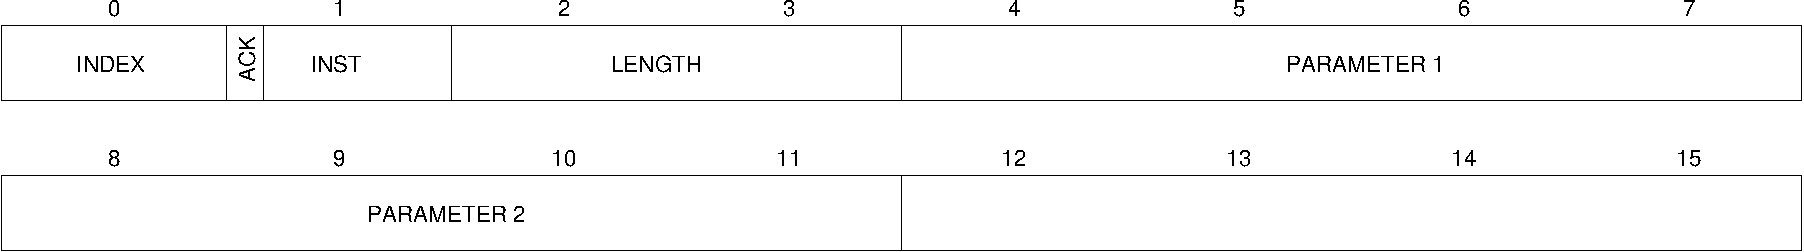
\includegraphics[width=16cm]{ethio.pdf}}
  \caption{\label{fig-ethio}Ethernet-IOBUS instruction format.}
\end{figure}

The first octet in the instruction is an index that numbers the instructions
in the packet consecutively starting from 1.  The end of the instruction list
is indicated by a zero octet.  

The second octet contains an instruction code.  The high bit is clear for a
request and is set in the acknowledgment.  The next two octets indicate the
number of octets of parameters that follow.  All data words are transmitted
with most-significant bits sent first.  Table~\ref{tab-ethio} lists the
instruction codes and the data sent as arguments and returned in
acknowledgments.
\begin{table}
  \begin{center}
    \begin{tabular}{|c|c|c|l|} \hline
  instruction & code & length & parameters  \\ \hline
write & 0x01 & 8 & 32-bit address, 32-bit data \\
write ack & 0x81 & 0 & -- \\ \hline
set & 0x02 & 8 & 32-bit address, 32-bit mask of bits to set \\
set ack & 0x82 & 0 & -- \\ \hline
read & 0x04 & 4 & 32-bit address \\
read ack & 0x84 & 8 & 32-bit address, 32-bit data \\ \hline
reset & 0x05 & 8 & 32-bit address, 32-bit mask of bits to clear \\
reset ack & 0x85 & 0 & -- \\ \hline
waitclr & 0x07 & 12 & 32-bit address, 32-bit mask of bits to test, \\
        &      &    & 32-bit timeout loop count \\
waitclr ack & 0x87 & 4 & actual loop count until bits were cleared \\ \hline
waitset & 0x08 & 12 & 32-bit address, 32-bit mask of bits to test, \\
        &      &    & 32-bit timeout loop count \\
waitset ack & 0x88 & 4 & actual loop count until bits were set \\ \hline
    \end{tabular}
  \end{center}
\caption{\label{tab-ethio}Instruction codes for the Ethernet-IOBUS protocol.}
\end{table}

\subsection{Discussion}
The UDP protocol is described as ``unreliable'' in the sense that it
provides no guarantee that data will be delivered, that it will be received
or that it will be processed correctly.  Any reliability requirements must
be built into a higher level protocol that uses UDP as the mechanism for
data transfer.  The other end of the spectrum is TCP, which provides
extensive mechanisms for determining whether data has been received and
successfully delivered to a user application, and for retransmitting packets
that may not have been received.  Furthermore, TCP achieves high bandwidth
utilization by sending packets before receiving acknowledgments of previously
transmitted packets.  Any packets that are retransmitted could arrive out of
order and would need to be reassembled into the correct sequence by the
receiver.  This functionality requires a significant amount of overhead for
buffering data and maintaining lists of received and acknowledged packets.

In contrast, the TFTP protocol uses UDP to send data, with the receiver
acknowledging each packet that is correctly received and processed while the
transmitter waits for the acknowledgments before transmitting the next packet.
This achieves low latency except when packets are lost, which incurrs a delay
due to the timeout when waiting for the acknowledgement.

The main reliability requirements for the ETHIO protocol are as follows:
\begin{itemize}
  \item Packets should be acknowledged, but the transmitter may choose to
        ignore the acknowledgment if guaranteed reliability is not necessary
  \item Duplicate packets should be acknowledged but not processed
\end{itemize}
Currently, the protocol addresses the first, but not the second requirement.
The addition of a packet sequence number in the header would be sufficient
to keep track of which packets have been processed, as is done in the TFTP
protocol.

\subsubsection{Collisions}
The GbE interface can provide multiple clients for receiving UDP packets
but the simplest instantiation includes one client that receives all UDP
traffic.  This creates the potential for collisions, whereby one packet's
payload is overwritten by an incomming packet either beofre or as it is being
processed.  There are several ways that this possibility can be mitigated:
\begin{itemize}
  \item Only buffer packets with a matching destination port, discarding
        all others
  \item Provide multiple UDP clients that buffer packets based on
        different destination ports
  \item Double buffer the incomming and delivered data
\end{itemize}

\appendix
\section{Connector Nets}
\begin{table}
\begin{center}
\scriptsize
\begin{tabular}{|c|r|l|c|} \hline
\multicolumn{4}{|c|}{Channel 0 - Connector J4} \\ \hline
pin & CAPTAN net & STIB net & pad \\ \hline\hline
 1 &                   & PULSE\_IN\_D2              &    \\
 2 &                   & A\_M4\_GND                 &    \\ \hline
 3 &                   & A\_M4\_GND                 &    \\
 4 &                   & A\_M4\_GND                 &    \\ \hline
 5 & BUSDHS\_01DP\_02S & STRIP\_GOTHITOR\_PAD\_P[0] & B13 \\
 6 & BUSDHS\_01DN\_03S & STRIP\_GOTHITOR\_PAD\_N[0] & B12 \\ \hline
 7 &                   & A\_M4\_GND                 &    \\
 8 &                   & A\_M4\_GND                 &    \\ \hline
 9 & BUSDHS\_02DP\_04S & STRIP\_OUT2\_4\_PAD\_P[0]  & A16 \\
10 & BUSDHS\_02DN\_05S & STRIP\_OUT2\_4\_PAD\_N[0]  & A15 \\ \hline
11 &                   & A\_M4\_GND &    \\
12 &                   & A\_M4\_GND &    \\ \hline
13 &   BUSB\_10DP\_20S & STRIP\_MCLKA\_PAD\_P       & AA7 \\
14 &   BUSB\_10DN\_21S & STRIP\_MCLKA\_PAD\_N       & Y7 \\ \hline
15 & BUSDHS\_03DP\_06S & STRIP\_OUT2\_3\_PAD\_P[0]  &  A10 \\
16 & BUSDHS\_03DN\_07S & STRIP\_OUT2\_3\_PAD\_N[0]  &  B10 \\ \hline
17 & BUSDHS\_04DP\_08S & STRIP\_OUT2\_2\_PAD\_P[0]  &  K26 \\
18 & BUSDHS\_04DN\_09S & STRIP\_OUT2\_2\_PAD\_N[0]  &  K25 \\ \hline
19 &   BUSB\_07DP\_14S & STRIP\_MCLKB\_PAD\_P       & V4   \\
20 &   BUSB\_07DN\_15S & STRIP\_MCLKB\_PAD\_N       & U4   \\ \hline
21 &                   & A\_M4\_GND &      \\
22 &                   & A\_M4\_GND &      \\ \hline
23 &GENERAL\_05DP\_10S & STRIP\_OUT2\_1\_PAD\_P[0]  &  C13 \\
24 &GENERAL\_05DN\_11S & STRIP\_OUT2\_1\_PAD\_N[0]  &  C12 \\ \hline
25 &   BUSD\_21DP\_42S & STRIP\_BCOCLK\_PAD\_P[0]   & H22 \\
26 &   BUSD\_21DN\_43S & STRIP\_BCOCLK\_PAD\_N[0]   & H21 \\ \hline
27 &   BUSD\_20DP\_40S & STRIP\_OUT1\_4\_PAD\_P[0]  &  D24 \\
28 &   BUSD\_20DN\_41S & STRIP\_OUT1\_4\_PAD\_N[0]  &  C24 \\ \hline
29 &   BUSD\_19DP\_38S & STRIP\_OUT2\_0\_PAD\_P[0]  &  A22 \\
30 &   BUSD\_19DN\_39S & STRIP\_OUT2\_0\_PAD\_N[0]  &  A21 \\ \hline
31 &                   & A\_M4\_GND & \\
32 &                   & A\_M4\_GND & \\ \hline
33 &   BUSD\_18DP\_36S & STRIP\_OUT1\_3\_PAD\_P[0]  &  D22 \\
34 &   BUSD\_18DN\_37S & STRIP\_OUT1\_3\_PAD\_N[0]  &  C22 \\ \hline
35 &   BUSD\_17DP\_34S & STRIP\_SCIN\_PAD\_P[0]     & A20 \\
36 &   BUSD\_17DN\_35S & STRIP\_SCIN\_PAD\_N[0]     & A19 \\ \hline
37 &   BUSD\_16DP\_32S & STRIP\_SHIFT\_PAD\_P[0]    & E21 \\
38 &   BUSD\_16DN\_33S & STRIP\_SHIFT\_PAD\_N[0]    & D21 \\ \hline
39 &   BUSD\_31DP\_62S & STRIP\_OUT1\_2\_PAD\_P[0]  &  K24 \\
40 &   BUSD\_31DN\_63S & STRIP\_OUT1\_2\_PAD\_N[0]  &  K23 \\ \hline
41 &                   & A\_M4\_GND & \\
42 &                   & A\_M4\_GND & \\ \hline
43 &   BUSD\_30DP\_60S & STRIP\_RESET\_PAD\_P[0]    & J21 \\
44 &   BUSD\_30DN\_32S & STRIP\_RESET\_PAD\_N[0]    & J20 \\ \hline
45 &   BUSD\_29DP\_58S & STRIP\_OUT1\_1\_PAD\_P[0]  &  J23 \\
46 &   BUSD\_29DN\_58S & STRIP\_OUT1\_1\_PAD\_N[0]  &  J22 \\ \hline
47 &   BUSD\_28DP\_56S & STRIP\_SCOUT\_PAD\_P[0]    & J26 \\
48 &   BUSD\_28DN\_57S & STRIP\_SCOUT\_PAD\_N[0]    & J25 \\ \hline
49 &   BUSD\_27DP\_54S & STRIP\_OUT1\_0\_PAD\_P[0]  &  H26 \\
50 &   BUSD\_27DN\_55S & STRIP\_OUT1\_0\_PAD\_N[0]  &  H25 \\ \hline
\end{tabular}
\end{center}
\end{table}

\begin{table}
\begin{center}
\scriptsize
\begin{tabular}{|c|r|l|c|l|} \hline
\multicolumn{5}{|c|}{Channel 1 - Connector J3} \\ \hline
pin & CAPTAN net    & STIB net & pad & notes \\ \hline\hline
 1 &               & PULSE\_IN\_D1  & & \\
 2 &               & A\_M3\_GND  & & \\ \hline
 3 &               & A\_M3\_GND & & \\
 4 &               & A\_M3\_GND & & \\ \hline
 5 & BUSD\_12DP\_24S & STRIP\_GOTHITOR\_PAD\_P[1] & H20 & \\
 6 & BUSD\_12DN\_25S & STRIP\_GOTHITOR\_PAD\_N[1] & G20 & \\ \hline
 7 &               & A\_M3\_GND                &   &   \\
 8 &               & A\_M3\_GND                &    &  \\ \hline
 9 & BUSD\_11DP\_22S & STRIP\_OUT2\_4\_PAD\_P[1]   & D23&  \\
10 & BUSD\_11DN\_23S & STRIP\_OUT2\_4\_PAD\_N[1]   & C23&  \\ \hline
11 &      A\_M3\_GND &                         &    &  \\
12 &      A\_M3\_GND &                         &    &  \\ \hline
13 & BUSB\_10DP\_20S & STRIP\_MCLKA\_PAD\_P       & AA7&  \\
14 & BUSB\_10DN\_21S & STRIP\_MCLKA\_PAD\_N       & Y7&  \\ \hline
15 & BUSD\_10DP\_20S & STRIP\_OUT2\_3\_PAD\_P[1]   & C26 & \\
16 & BUSD\_10DN\_21S & STRIP\_OUT2\_3\_PAD\_N[1]   & C25 & \\ \hline
17 & BUSD\_09DP\_18S & STRIP\_OUT2\_2\_PAD\_P[1]   & F20 & \\
18 & BUSD\_09DN\_19S & STRIP\_OUT2\_2\_PAD\_N[1]   & E20 & \\ \hline
19 & BUSB\_07DP\_14S & STRIP\_MCLKB\_PAD\_P       & V4 & \\
20 & BUSB\_07DN\_15S & STRIP\_MCLKB\_PAD\_N       & U4 & \\ \hline
21 &               & A\_M3\_GND                &    & \\
22 &               & A\_M3\_GND                &    & \\ \hline
23 & BUSD\_08DP\_16S & STRIP\_OUT2\_1\_PAD\_P[1]   & E23 & \\
24 & BUSD\_08DN\_17S & STRIP\_OUT2\_1\_PAD\_N[1]   & E22 & \\ \hline
25 & GENERAL\_02DP\_04S & STRIP\_BCOCLK\_PAD\_P[1] & \sout{G18} & IO\_L9P\_CC\_LC\_5 \\
26 & GENERAL\_02DN\_05S & STRIP\_BCOCLK\_PAD\_N[1] & \sout{G17} &IO\_L9N\_CC\_LC\_5 \\ \hline
27 &  BUSD\_07DP\_14S & STRIP\_OUT1\_4\_PAD\_P[1]  & M23 & \\
28 &  BUSD\_07DN\_15S & STRIP\_OUT1\_4\_PAD\_N[1]  & M22 & \\ \hline
29 &  BUSD\_06DP\_12S & STRIP\_OUT2\_0\_PAD\_P[1]  & M21 & \\
30 &  BUSD\_06DN\_13S & STRIP\_OUT2\_0\_PAD\_N[1]  & M20 & \\ \hline
31 &                & A\_M3\_GND               &     & \\
32 &                & A\_M3\_GND               &     & \\ \hline
33 &  BUSD\_05DP\_10S & STRIP\_OUT1\_3\_PAD\_P[1]  & L26 & \\
34 &  BUSD\_05DN\_11S & STRIP\_OUT1\_3\_PAD\_N[1]  & M26 & \\ \hline
35 & GENERAL\_03DP\_06S & STRIP\_SCIN\_PAD\_P[1]  & \sout{D26}& IO\_L25P\_CC\_LC\_5 \\
36 & GENERAL\_03DN\_07S & STRIP\_SCIN\_PAD\_N[1]  & \sout{D25}& IO\_L25N\_CC\_LC\_5  \\ \hline
37 & GENERAL\_04DP\_08S & STRIP\_SHIFT\_PAD\_P[1] & \sout{B17} & IO\_L7P\_GC\_LC\_3 \\
38 & GENERAL\_04DN\_09S & STRIP\_SHIFT\_PAD\_N[1] & \sout{A17} & IO\_L7N\_GC\_LC\_3  \\ \hline
39 &  BUSD\_04DP\_08S & STRIP\_OUT1\_2\_PAD\_P[1]  & M25 & \\
40 &  BUSD\_04DN\_09S & STRIP\_OUT1\_2\_PAD\_N[1]  & M24 & \\ \hline
41 &                & A\_M3\_GND               &     & \\
42 &                & A\_M3\_GND               &     & \\ \hline
43 &  BUSD\_03DP\_06S & STRIP\_RESET\_PAD\_P[1]   &  L24 & \\
44 &  BUSD\_03DN\_07S & STRIP\_RESET\_PAD\_N[1]   &  L23 & \\ \hline
45 &  BUSD\_02DP\_04S & STRIP\_OUT1\_1\_PAD\_P[1]  &  L21 & \\
46 &  BUSD\_02DN\_05S & STRIP\_OUT1\_1\_PAD\_N[1]  &  L20 & \\ \hline
47 &  BUSD\_01DP\_02S & STRIP\_SCOUT\_PAD\_P[1]   &  L19 & \\
48 &  BUSD\_01DN\_03S & STRIP\_SCOUT\_PAD\_N[1]   &  K20 & \\ \hline
49 &  BUSD\_00DP\_00S & STRIP\_OUT1\_0\_PAD\_P[1]  &  K22 & \\
50 &  BUSD\_00DN\_01S & STRIP\_OUT1\_0\_PAD\_N[1]  &  K21 & \\ \hline
\end{tabular}
\end{center}
\end{table}

\begin{table}
\begin{center}
\scriptsize
\begin{tabular}{|c|r|l|c|} \hline
\multicolumn{4}{|c|}{Channel 2 - Connector J8} \\ \hline
pin & CAPTAN net    & STIB net & pad \\ \hline\hline
 1 &                  &  PULSE\_IN\_C2            & \\
 2 &                  &  A\_M2\_GND               & \\ \hline
 3 &                  &  A\_M2\_GND               & \\
 4 &                  &  A\_M2\_GND               & \\ \hline
 5 &  BUSCHS\_04DP\_08S &  STRIP\_GOTHITOR\_PAD\_P[2] & R20 \\
 6 &  BUSCHS\_04DN\_09S &  STRIP\_GOTHITOR\_PAD\_N[2] & R19 \\ \hline
 7 &                  &  A\_M2\_GND               & \\
 8 &                  &  A\_M2\_GND               & \\ \hline
 9 & GENERAL\_23DP\_46S &  STRIP\_OUT2\_4\_PAD\_P[2]   & AC13 \\
10 & GENERAL\_23DN\_47S &  STRIP\_OUT2\_4\_PAD\_N[2]   & AD13 \\ \hline
11 &                  &  A\_M2\_GND               & \\
12 &                  &  A\_M2\_GND               & \\ \hline
13 &    BUSB\_10DP\_20S &  STRIP\_MCLKA\_PAD\_P       & AA7 \\
14 &    BUSB\_10DN\_21S &  STRIP\_MCLKA\_PAD\_N       & Y7 \\ \hline
15 &    BUSC\_11DP\_22S &  STRIP\_OUT2\_3\_PAD\_P[2]   & AA18 \\
16 &    BUSC\_11DN\_23S &  STRIP\_OUT2\_3\_PAD\_N[2]   & Y18 \\ \hline
17 &    BUSC\_10DP\_20S &  STRIP\_OUT2\_2\_PAD\_P[2]   & Y20 \\
18 &    BUSC\_10DN\_21S &  STRIP\_OUT2\_2\_PAD\_N[2]   & Y21 \\ \hline
19 &    BUSB\_07DP\_14S &  STRIP\_MCLKB\_PAD\_P       & V4 \\
20 &    BUSB\_07DN\_15S &  STRIP\_MCLKB\_PAD\_N       & U4 \\ \hline
21 &                  &  A\_M2\_GND               & \\
22 &                  &  A\_M2\_GND               & \\ \hline
23 &    BUSC\_08DP\_16S &  STRIP\_OUT2\_1\_PAD\_P[2]   & Y19 \\
24 &    BUSC\_08DN\_17S &  STRIP\_OUT2\_1\_PAD\_N[2]   & W19 \\ \hline
25 &    BUSC\_07DP\_14S &  STRIP\_BCOCLK\_PAD\_P[2]   & AF19 \\
26 &    BUSC\_07DN\_15S &  STRIP\_BCOCLK\_PAD\_N[2]   & AF20 \\ \hline
27 &    BUSC\_06DP\_12S &  STRIP\_OUT1\_4\_PAD\_P[2]   & AE21 \\
28 &    BUSC\_06DN\_13S &  STRIP\_OUT1\_4\_PAD\_N[2]   & AD21 \\ \hline
29 &    BUSC\_05DP\_10S &  STRIP\_OUT2\_0\_PAD\_P[2]   & AF18 \\
30 &    BUSC\_05DN\_11S &  STRIP\_OUT2\_0\_PAD\_N[2]   & AE18 \\ \hline
31 &                  &  A\_M2\_GND               & \\
32 &                  &  A\_M2\_GND               & \\ \hline
33 & GENERAL\_18DP\_36S &  STRIP\_OUT1\_3\_PAD\_P[2]   & AA16 \\
34 & GENERAL\_18DN\_37S &  STRIP\_OUT1\_3\_PAD\_N[2]   & AA15 \\ \hline
35 &    BUSC\_04DP\_08S &  STRIP\_SCIN\_PAD\_P[2]     & AF21 \\
36 &    BUSC\_04DN\_09S &  STRIP\_SCIN\_PAD\_N[2]     & AF22 \\ \hline
37 &    BUSC\_03DP\_06S &  STRIP\_SHIFT\_PAD\_P[2]    & AC18 \\
38 &    BUSB\_03DN\_07S &  STRIP\_SHIFT\_PAD\_N[2]    & AB18 \\ \hline
39 & GENERAL\_19DP\_38S &  STRIP\_OUT1\_2\_PAD\_P[2]   & AB13 \\
40 & GENERAL\_19DN\_39S &  STRIP\_OUT1\_2\_PAD\_N[2]   & AA13 \\ \hline
41 &                  &  A\_M2\_GND               & \\
42 &                  &  A\_M2\_GND               & \\ \hline
43 &    BUSC\_02DP\_04S &  STRIP\_RESET\_PAD\_P[2]    & AB20 \\
44 &    BUSC\_02DN\_05S &  STRIP\_RESET\_PAD\_N[2]    & AC20 \\ \hline
45 & GENERAL\_20DP\_40S &  STRIP\_OUT1\_1\_PAD\_P[2]   & AC14 \\
46 & GENERAL\_20DN\_41S &  STRIP\_OUT1\_1\_PAD\_N[2]   & AD14 \\ \hline
47 & GENERAL\_21DP\_42S &  STRIP\_SCOUT\_PAD\_P[2]    & AA12 \\
48 & GENERAL\_21DN\_43S &  STRIP\_SCOUT\_PAD\_N[2]    & AA11 \\ \hline
49 & GENERAL\_22DP\_44S &  STRIP\_OUT1\_0\_PAD\_P[2]   & AC16 \\ 
50 & GENERAL\_22DN\_45S &  STRIP\_OUT1\_0\_PAD\_N[2]   & AC15 \\ \hline
\end{tabular}
\end{center}
\end{table}

\begin{table}
\begin{center}
\scriptsize
\begin{tabular}{|c|r|l|c|l|} \hline
\multicolumn{5}{|c|}{Channel 3 - Connector J7} \\ \hline
pin & CAPTAN net    & STIB net & pad & notes \\ \hline\hline
 1 &                 & PULSE\_IN\_C1             &  & \\
 2 &                 & A\_M1\_GND                &  & \\ \hline
 3 &                 & A\_M1\_GND                &  & \\
 4 &                 & A\_M1\_GND                &  & \\ \hline
 5 &  BUSCC\_00DP\_00S & STRIP\_GOTHITOR\_PAD\_P[3] & P20  & \\
 6 &  BUSCC\_00DN\_00S & STRIP\_GOTHITOR\_PAD\_N[3] & P19  & \\ \hline
 7 &                 & A\_M1\_GND                &  & \\
 8 &                 & A\_M1\_GND                &  & \\ \hline
 9 &  BUSCC\_01DP\_02S & STRIP\_OUT2\_4\_PAD\_P[3]   & R24  & \\
10 &  BUSCC\_01DN\_03S & STRIP\_OUT2\_4\_PAD\_N[3]   & R23  & \\ \hline
11 &                 & A\_M1\_GND                &  & \\
12 &                 & A\_M1\_GND                &  & \\ \hline
13 &   BUSB\_10DP\_20S & STRIP\_MCLKA\_PAD\_P       & AA7  & \\
14 &   BUSB\_10DN\_21S & STRIP\_MCLKA\_PAD\_N       & Y7   & \\ \hline
15 &  BUSCC\_02DP\_04S & STRIP\_OUT2\_3\_PAD\_P[3]   & R22 & \\
16 &  BUSCC\_02DN\_05S & STRIP\_OUT2\_3\_PAD\_N[3]   & R21 & \\ \hline
17 &  BUSCC\_03DP\_06S & STRIP\_OUT2\_2\_PAD\_P[3]   & T26 & \\
18 &  BUSCC\_03DN\_07S & STRIP\_OUT2\_2\_PAD\_N[3]   & U26 & \\ \hline
19 &   BUSB\_07DP\_14S & STRIP\_MCLKB\_PAD\_P       & V4 & \\
20 &   BUSB\_07DN\_15S & STRIP\_MCLKB\_PAD\_N       & U4 & \\ \hline
21 &                 & A\_M1\_GND                & & \\
22 &                 & A\_M1\_GND                & & \\ \hline
23 &  BUSCC\_04DP\_08S & STRIP\_OUT2\_1\_PAD\_P[3]   & U23 & \\
24 &  BUSCC\_04DN\_09S & STRIP\_OUT2\_1\_PAD\_N[3]   & V23 & \\ \hline
25 &   BUSC\_31DP\_62S & STRIP\_BCOCLK\_PAD\_P[3]   & R26 & \\
26 &   BUSC\_31DN\_63S & STRIP\_BCOCLK\_PAD\_N[3]   & R25 & \\ \hline
27 &  BUSCC\_05DP\_10S & STRIP\_OUT1\_4\_PAD\_P[3]   & U25 & \\
28 &  BUSCC\_05DN\_11S & STRIP\_OUT1\_4\_PAD\_N[3]   & U24 & \\ \hline
29 &  BUSCC\_06DP\_12S & STRIP\_OUT2\_0\_PAD\_P[3]   & U22 & \\
30 &  BUSCC\_06DN\_13S & STRIP\_OUT2\_0\_PAD\_N[3]   & U21 & \\ \hline
31 &                 & A\_M1\_GND                & & \\
32 &                 & A\_M1\_GND                & & \\ \hline
33 &  BUSCC\_07DP\_14S & STRIP\_OUT1\_3\_PAD\_P[3]   & T21 & \\
34 &  BUSCC\_07DN\_15S & STRIP\_OUT1\_3\_PAD\_N[3]   & T20 & \\ \hline
35 &   BUSC\_30DP\_60S & STRIP\_SCIN\_PAD\_P[3]     & P23 & \\
36 &   BUSC\_30DN\_61S & STRIP\_SCIN\_PAD\_N[3]     & P22 & \\ \hline
37 &   BUSC\_29DP\_58S & STRIP\_SHIFT\_PAD\_P[3]    & P25 & \\
38 &   BUSB\_29DN\_59S & STRIP\_SHIFT\_PAD\_N[3]    & P24 & \\ \hline
39 & BUSCHS\_00DP\_00S & STRIP\_OUT1\_2\_PAD\_P[3]   & \sout{AD19} & IO\_L25P\_CC\_SM7\_LC\_7 \\
40 & BUSCHS\_00DN\_01S & STRIP\_OUT1\_2\_PAD\_N[3]   & \sout{AC19} & IO\_L25N\_CC\_SM7\_LC\_7 \\ \hline
41 &                 & A\_M1\_GND                & & \\
42 &                 & A\_M1\_GND                & & \\ \hline
43 &   BUSC\_28DP\_56S & STRIP\_RESET\_PAD\_P[3]    & N21 & \\
44 &   BUSC\_28DN\_57S & STRIP\_RESET\_PAD\_N[3]    & N20 & \\ \hline
45 & BUSCHS\_01DP\_02S & STRIP\_OUT1\_1\_PAD\_P[3]   & \sout{AC21} & IO\_L24P\_CC\_LC\_7  \\
46 & BUSCHS\_01DN\_03S & STRIP\_OUT1\_1\_PAD\_N[3]   & \sout{AB21} & IO\_L24N\_CC\_LC\_7 \\ \hline
47 & BUSCHS\_02DP\_04S & STRIP\_SCOUT\_PAD\_P[3]    & \sout{AA24} & IO\_L8P\_CC\_LC\_7 \\
48 & BUSCHS\_02DN\_05S & STRIP\_SCOUT\_PAD\_N[3]    & \sout{Y24} & IO\_L8N\_CC\_LC\_7 \\  \hline
49 & BUSCHS\_03DP\_06S & STRIP\_OUT1\_0\_PAD\_P[3]   & \sout{AC25} & IO\_L9P\_CC\_LC\_7 \\
50 & BUSCHS\_03DN\_07S & STRIP\_OUT1\_0\_PAD\_N[3]   & \sout{AC26} & IO\_L9N\_CC\_LC\_7 \\ \hline
\end{tabular}
\end{center}
\end{table}


\begin{table}
\begin{center}
\scriptsize
\begin{tabular}{|c|r|l|c|} \hline
\multicolumn{4}{|c|}{Channel 4 - Connector J19} \\ \hline
pin & CAPTAN net & STIB net & pad \\ \hline\hline
 1 &                 &  PULSE\_IN\_B2             &      \\
 2 &                 &  B\_M1\_GND                &      \\ \hline
 3 &                 &  B\_M1\_GND                &      \\
 4 &                 &  B\_M1\_GND                &      \\ \hline
 5 & BUSBHS\_03DP\_06S &  STRIP\_GOTHITOR\_PAD\_P[4] & AE10 \\
 6 & BUSBHS\_03DN\_07S &  STRIP\_GOTHITOR\_PAD\_N[4] & AD10 \\ \hline
 7 &                 &  B\_M1\_GND                &      \\
 8 &                 &  B\_M1\_GND                &      \\ \hline
 9 & BUSBHS\_04DP\_08S &  STRIP\_OUT2\_4\_PAD\_P[4]   & AD17 \\
10 & BUSBHS\_04DN\_08S &  STRIP\_OUT2\_4\_PAD\_N[4]   & AD16 \\ \hline
11 &                 &  B\_M1\_GND                &      \\
12 &                 &  B\_M1\_GND                &      \\ \hline
13 &   BUSB\_10DP\_20S &  STRIP\_MCLKA\_PAD\_P       & AA7  \\
14 &   BUSB\_10DN\_21S &  STRIP\_MCLKA\_PAD\_N       & Y7   \\ \hline
15 &\sout{GENERAL\_17DP\_34S} &  STRIP\_OUT2\_3\_PAD\_P[4]   & ---  \\
16 &GENERAL\_17DN\_35S &  STRIP\_OUT2\_3\_PAD\_N[4]   & AD11  \\ \hline
17 &   BUSB\_22DP\_44S &  STRIP\_OUT2\_2\_PAD\_P[4]   & AC4  \\
18 &   BUSB\_22DN\_45S &  STRIP\_OUT2\_2\_PAD\_N[4]   & AB4  \\ \hline
19 &   BUSB\_07DP\_14S &  STRIP\_MCLKB\_PAD\_P       & V4  \\
20 &   BUSB\_07DN\_15S &  STRIP\_MCLKB\_PAD\_N       & U4  \\ \hline
21 &                 &  B\_M1\_GND                &      \\
22 &                 &  B\_M1\_GND                &      \\ \hline
23 &   BUSB\_20DP\_40S &  STRIP\_OUT2\_1\_PAD\_P[4]   & AA4  \\
24 &   BUSB\_20DN\_41S &  STRIP\_OUT2\_1\_PAD\_N[4]   & AA3  \\ \hline
25 &   BUSB\_19DP\_38S &  STRIP\_BCOCLK\_PAD\_P[4]   & Y2  \\
26 &   BUSB\_19DN\_39S &  STRIP\_BCOCLK\_PAD\_N[4]   & Y1  \\ \hline
27 &   BUSB\_18DP\_36S &  STRIP\_OUT1\_4\_PAD\_P[4]   & W6  \\
28 &   BUSB\_18DN\_37S &  STRIP\_OUT1\_4\_PAD\_N[4]   & W5  \\ \hline
29 &   BUSB\_17DP\_34S &  STRIP\_OUT2\_0\_PAD\_P[4]   & W4  \\
30 &   BUSB\_17DN\_35S &  STRIP\_OUT2\_0\_PAD\_N[4]   & W3  \\ \hline
31 &                 &  B\_M1\_GND                &      \\
32 &                 &  B\_M1\_GND                &      \\ \hline
33 &   BUSB\_16DP\_32S &  STRIP\_OUT1\_3\_PAD\_P[4]   & W7  \\
34 &   BUSB\_16DN\_33S &  STRIP\_OUT1\_3\_PAD\_N[4]   & V7  \\ \hline
35 &   BUSB\_31DP\_62S &  STRIP\_SCIN\_PAD\_P[4]     & R4  \\
36 &   BUSB\_31DN\_63S &  STRIP\_SCIN\_PAD\_N[4]     & R3  \\ \hline
37 &   BUSB\_30DP\_60S &  STRIP\_SHIFT\_PAD\_P[4]    & P8  \\
38 &   BUSB\_30DN\_61S &  STRIP\_SHIFT\_PAD\_N[4]    & N8  \\ \hline
39 &   BUSB\_29DP\_58S &  STRIP\_OUT1\_2\_PAD\_P[4]   & P5  \\
40 &   BUSB\_29DN\_59S &  STRIP\_OUT1\_2\_PAD\_N[4]   & P4  \\ \hline
41 &                 &  B\_M1\_GND                &      \\
42 &                 &  B\_M1\_GND                &      \\ \hline
43 &   BUSB\_28DP\_56S &  STRIP\_RESET\_PAD\_P[4]    & U6  \\
44 &   BUSB\_28DN\_57S &  STRIP\_RESET\_PAD\_N[4]    & U5  \\ \hline
45 &   BUSB\_27DP\_54S &  STRIP\_OUT1\_1\_PAD\_P[4]   & AD2  \\
46 &   BUSB\_27DN\_55S &  STRIP\_OUT1\_1\_PAD\_N[4]   & AD1  \\ \hline
47 &   BUSB\_26DP\_52S &  STRIP\_SCOUT\_PAD\_P[4]    & AF3  \\
48 &   BUSB\_26DN\_51S &  STRIP\_SCOUT\_PAD\_N[4]    & AE3  \\ \hline
49 &   BUSB\_25DP\_50S &  STRIP\_OUT1\_0\_PAD\_P[4]   & AC2  \\
50 &   BUSB\_25DN\_49S &  STRIP\_OUT1\_0\_PAD\_N[4]   & AC1  \\ \hline
\end{tabular}
\end{center}
\end{table}


\begin{table}
\begin{center}
\scriptsize
\begin{tabular}{|c|r|l|c|} \hline
\multicolumn{4}{|c|}{Channel 5 - Connector J20} \\ \hline
pin & CAPTAN net & STIB net & pad \\ \hline\hline
 1 &                & PULSE\_IN\_B1 & \\
 2 &                & B\_M2\_GND & \\ \hline
 3 &                & B\_M2\_GND & \\
 4 &                & B\_M2\_GND & \\ \hline
 5 &  BUSB\_12DP\_24S & STRIP\_GOTHITOR\_PAD\_P[6] & AD5 \\
 6 &  BUSB\_12DN\_25S & STRIP\_GOTHITOR\_PAD\_N[6] &  AD4 \\ \hline
 7 &                & B\_M2\_GND & \\
 8 &                & B\_M2\_GND & \\ \hline
 9 &  BUSB\_11DP\_22S & STRIP\_OUT2\_4\_PAD\_P[6] & AA9 \\
10 &  BUSB\_11DN\_23S & STRIP\_OUT2\_4\_PAD\_N[6] &  Y9 \\ \hline
11 &                & B\_M2\_GND & \\
12 &                & B\_M2\_GND & \\ \hline
13 &  BUSB\_10DP\_20S & STRIP\_MCLKA\_PAD\_P     &   AA7 \\
14 &  BUSB\_10DN\_21S & STRIP\_MCLKA\_PAD\_N     &   Y7 \\ \hline
15 &  BUSB\_09DP\_18S & STRIP\_OUT2\_3\_PAD\_P[6] &   AF6 \\
16 &  BUSB\_09DN\_19S & STRIP\_OUT2\_3\_PAD\_N[6] &   AF5 \\ \hline
17 &  BUSB\_08DP\_16S & STRIP\_OUT2\_2\_PAD\_P[6] &   AD3 \\
18 &  BUSB\_08DN\_17S & STRIP\_OUT2\_2\_PAD\_N[6] &   AC3 \\ \hline
19 &  BUSB\_07DP\_14S & STRIP\_MCLKB\_PAD\_P     &   V4 \\
20 &  BUSB\_07DN\_15S & STRIP\_MCLKB\_PAD\_N     &   U4 \\ \hline
21 &                & B\_M2\_GND & \\
22 &                & B\_M2\_GND & \\ \hline
23 &  BUSB\_06DP\_12S & STRIP\_OUT2\_1\_PAD\_P[6] &   U3 \\
24 &  BUSB\_06DN\_13S & STRIP\_OUT2\_1\_PAD\_N[6] &   U2 \\ \hline
25 &  BUSB\_05DP\_10S & STRIP\_BCOCLK\_PAD\_P[6] &   T7 \\
26 &  BUSB\_06DP\_11S & STRIP\_BCOCLK\_PAD\_N[6] &   T6 \\ \hline
27 &  BUSB\_04DP\_08S & STRIP\_OUT1\_4\_PAD\_P[6] &   T4 \\
28 &  BUSB\_04DN\_09S & STRIP\_OUT1\_4\_PAD\_N[6] &   T3 \\ \hline
29 &  BUSB\_03DP\_06S & STRIP\_OUT2\_0\_PAD\_P[6] &   P3 \\
30 &  BUSB\_03DN\_07S & STRIP\_OUT2\_0\_PAD\_N[6] &   P2 \\ \hline
31 &                & B\_M2\_GND & \\
32 &                & B\_M2\_GND & \\ \hline
33 & GENERAL\_12DP\_24S & STRIP\_OUT1\_3\_PAD\_P[6]  &  T24 \\
34 & GENERAL\_12DN\_25S & STRIP\_OUT1\_3\_PAD\_N[6]  &  T23 \\ \hline
35 &  BUSB\_02DP\_04S & STRIP\_SCIN\_PAD\_P[6]      & R6 \\
36 &  BUSB\_02DN\_05S & STRIP\_SCIN\_PAD\_N[6]    &   R5 \\ \hline
37 &  BUSB\_01DP\_02S & STRIP\_SHIFT\_PAD\_P[6]     & R2 \\
38 &  BUSB\_01DN\_03S & STRIP\_SHIFT\_PAD\_N[6]   &   R1 \\ \hline
39 & GENERAL\_13DP\_26S & STRIP\_OUT1\_2\_PAD\_P[6]     &AC6 \\
40 & GENERAL\_13DN\_27S & STRIP\_OUT1\_2\_PAD\_N[6]   &  AB6 \\ \hline
41 &                  & B\_M2\_GND & \\
42 &                  & B\_M2\_GND & \\ \hline
43 &  BUSB\_00DP\_00S   &  STRIP\_RESET\_PAD\_P[6]  &  P7 \\
44 &  BUSB\_00DN\_01S   &  STRIP\_RESET\_PAD\_N[6]  &  P6 \\ \hline
45 & GENERAL\_14DP\_28S   &  STRIP\_OUT1\_1\_PAD\_P[6] &  U20 \\
46 & GENERAL\_14DN\_29S   &  STRIP\_OUT1\_1\_PAD\_N[6] &  T19 \\ \hline
47 & GENERAL\_15DP\_30S   &  STRIP\_SCOUT\_PAD\_P[6]  &  V26 \\
48 & GENERAL\_15DN\_31S   &  STRIP\_SCOUT\_PAD\_N[6]  &  V25 \\ \hline
49 & GENERAL\_16DP\_32S   &  STRIP\_OUT1\_0\_PAD\_P[6] &  R8 \\
50 & GENERAL\_16DP\_32S   &  STRIP\_OUT1\_0\_PAD\_N[6] &  R7 \\ \hline
\end{tabular}
\end{center}
\end{table}


\begin{table}
\begin{center}
\scriptsize
\begin{tabular}{|c|r|l|c|} \hline
\multicolumn{4}{|c|}{Channel 6 - Connector J21} \\ \hline
pin & CAPTAN net & STIB net & pad \\ \hline\hline
 1 &                   & PULSE\_IN\_A2              &    \\
 2 &                   & B\_M3\_GND                 &    \\ \hline
 3 &                   & B\_M3\_GND                 &    \\
 4 &                   & B\_M3\_GND                 &    \\ \hline
 5 &   BUSA\_10DP\_20S & STRIP\_GOTHITOR\_PAD\_P[6] & C2 \\
 6 &   BUSA\_10DN\_21S & STRIP\_GOTHITOR\_PAD\_N[6] & C1 \\ \hline
 7 &                   & B\_M3\_GND                 &    \\
 8 &                   & B\_M3\_GND                 &    \\ \hline
 9 &   BUSA\_11DP\_22S & STRIP\_OUT2\_4\_PAD\_P[6]  & H8 \\
10 &   BUSA\_11DN\_23S & STRIP\_OUT2\_4\_PAD\_N[6]  & H7 \\ \hline
11 &                   & B\_M3\_GND                 &    \\
12 &                   & B\_M3\_GND                 &    \\ \hline
13 &   BUSB\_10DP\_20S & STRIP\_MCLKA\_PAD\_P       & AA7 \\
14 &   BUSB\_10DN\_21S & STRIP\_MCLKA\_PAD\_N       & Y7 \\ \hline
15 &   BUSA\_13DP\_26S & STRIP\_OUT2\_3\_PAD\_P[6]  & G6 \\
16 &   BUSA\_13DN\_27S & STRIP\_OUT2\_3\_PAD\_N[6]  & G5 \\ \hline
17 &   BUSA\_14DP\_28S & STRIP\_OUT2\_2\_PAD\_P[6]  & F8 \\
18 &   BUSA\_14DN\_29S & STRIP\_OUT2\_2\_PAD\_N[6]  & G8 \\ \hline
19 &   BUSB\_07DP\_14S & STRIP\_MCLKB\_PAD\_P       & V4 \\
20 &   BUSB\_07DN\_15S & STRIP\_MCLKB\_PAD\_N       & U4 \\ \hline
21 &                   & B\_M3\_GND                 &    \\
22 &                   & B\_M3\_GND                 &    \\ \hline
23 &   BUSA\_24DP\_48S & STRIP\_OUT2\_1\_PAD\_P[6]  & H6 \\
24 &   BUSA\_24DN\_49S & STRIP\_OUT2\_1\_PAD\_N[6]  & H5 \\ \hline
25 &   BUSA\_25DP\_50S & STRIP\_BCOCLK\_PAD\_P[6]   & G2 \\
26 &   BUSA\_25DN\_51S & STRIP\_BCOCLK\_PAD\_N[6]   & G1 \\ \hline
27 &   BUSA\_26DP\_52S & STRIP\_OUT1\_4\_PAD\_P[6]  & H4 \\
28 &   BUSA\_26DN\_53S & STRIP\_OUT1\_4\_PAD\_N[6]  & H3 \\ \hline
29 &   BUSA\_27DP\_54S & STRIP\_OUT2\_0\_PAD\_P[6]  & H2 \\
30 &   BUSA\_27DN\_55S & STRIP\_OUT2\_0\_PAD\_N[6]  & H1 \\ \hline
31 &                   & B\_M3\_GND                 & \\
32 &                   & B\_M3\_GND                 & \\ \hline
33 &   BUSA\_28DP\_56S & STRIP\_OUT1\_3\_PAD\_P[6]  & J2 \\
34 &   BUSA\_28DN\_57S & STRIP\_OUT1\_3\_PAD\_N[6]  & J1 \\ \hline
35 &   BUSA\_29DP\_58S & STRIP\_SCIN\_PAD\_P[6]     & J5 \\
36 &   BUSA\_29DN\_59S & STRIP\_SCIN\_PAD\_N[6]     & J4 \\ \hline
37 &   BUSA\_30DP\_60S & STRIP\_SHIFT\_PAD\_P[6]    & J7 \\
38 &   BUSA\_30DN\_61S & STRIP\_SHIFT\_PAD\_N[6]    & J6 \\ \hline
39 &   BUSA\_31DP\_62S & STRIP\_OUT1\_2\_PAD\_P[6]  & L1 \\
40 &   BUSA\_31DN\_63S & STRIP\_OUT1\_2\_PAD\_N[6]  & K1 \\ \hline
41 &                   & B\_M3\_GND                 & \\
42 &                   & B\_M3\_GND                 & \\ \hline
43 &   BUSA\_16DP\_32S & STRIP\_RESET\_PAD\_P[6]    & C5 \\
44 &   BUSA\_16DN\_32S & STRIP\_RESET\_PAD\_N[6]    & D5 \\ \hline
45 &   BUSA\_17DP\_34S & STRIP\_OUT1\_1\_PAD\_P[6]  & A9 \\
46 &   BUSA\_17DN\_35S & STRIP\_OUT1\_1\_PAD\_N[6]  & B9 \\ \hline
47 & GENERAL\_11DP\_22S & STRIP\_SCOUT\_PAD\_P[6]   & E13 \\
48 & GENERAL\_11DN\_23S & STRIP\_SCOUT\_PAD\_N[6]   & D12 \\ \hline
49 &  BUSAHS\_04DP\_08S & STRIP\_OUT1\_0\_PAD\_P[6] & L4 \\
50 &  BUSAHS\_04DN\_09S & STRIP\_OUT1\_0\_PAD\_N[6] & L3 \\ \hline
\end{tabular}
\end{center}
\end{table}

\begin{table}
\begin{center}
\scriptsize
\begin{tabular}{|c|r|l|c|} \hline
\multicolumn{4}{|c|}{Channel 7 - Connector J24} \\ \hline
pin & CAPTAN net & STIB net & pad \\ \hline\hline
 1 &                   & PULSE\_IN\_A1              &    \\
 2 &                   & B\_M4\_GND                 &    \\ \hline
 3 &                   & B\_M4\_GND                 &    \\
 4 &                   & B\_M4\_GND                 &    \\ \hline
 5 & BUSAHS\_03DP\_06S & STRIP\_GOTHITOR\_PAD\_P[7] & D2    \\
 6 & BUSAHS\_03DN\_07S & STRIP\_GOTHITOR\_PAD\_N[7] & D1    \\ \hline
 7 &                   & B\_M4\_GND                 &    \\
 8 &                   & B\_M4\_GND                 &    \\ \hline
 9 & BUSAHS\_02DP\_04S & STRIP\_OUT2\_4\_PAD\_P[7]  & G10    \\
10 & BUSAHS\_02DN\_05S & STRIP\_OUT2\_4\_PAD\_N[7]  & G9    \\ \hline
11 &                   & B\_M4\_GND                 &    \\
12 &                   & B\_M4\_GND                 &    \\ \hline
13 &   BUSB\_10DP\_20S & STRIP\_MCLKA\_PAD\_P       & AA7    \\
14 &   BUSB\_10DN\_21S & STRIP\_MCLKA\_PAD\_N       & Y7    \\ \hline
15 & BUSAHS\_01DP\_02S & STRIP\_OUT2\_3\_PAD\_P[7]  & E3    \\
16 & BUSAHS\_01DN\_03S & STRIP\_OUT2\_3\_PAD\_N[7]  & E2    \\ \hline
17 & BUSAHS\_00DP\_00S & STRIP\_OUT2\_2\_PAD\_P[7]  & B6    \\
18 & BUSAHS\_00DN\_01S & STRIP\_OUT2\_2\_PAD\_N[7]  & C6    \\ \hline
19 &   BUSB\_07DP\_14S & STRIP\_MCLKB\_PAD\_P       & V4    \\
20 &   BUSB\_07DN\_15S & STRIP\_MCLKB\_PAD\_N       & U4    \\ \hline
21 &                   & B\_M4\_GND                 &    \\
22 &                   & B\_M4\_GND                 &    \\ \hline
23 &  BUSAA\_07DP\_14S & STRIP\_OUT2\_1\_PAD\_P[7]  & N7    \\
24 &  BUSAA\_07DN\_15S & STRIP\_OUT2\_1\_PAD\_N[7]  & M7    \\ \hline
25 &   BUSA\_20DP\_40S & STRIP\_BCOCLK\_PAD\_P[7]   & C4    \\
26 &   BUSA\_20DN\_41S & STRIP\_BCOCLK\_PAD\_N[7]   & D4    \\ \hline
27 &  BUSAA\_06DP\_12S & STRIP\_OUT1\_4\_PAD\_P[7]  & M6    \\
28 &  BUSAA\_06DN\_13S & STRIP\_OUT1\_4\_PAD\_N[7]  & M5    \\ \hline
29 &  BUSAA\_05DP\_10S & STRIP\_OUT2\_0\_PAD\_P[7]  & M4    \\
30 &  BUSAA\_05DN\_11S & STRIP\_OUT2\_0\_PAD\_N[7]  & M3    \\ \hline
31 &                   & B\_M4\_GND                 &    \\
32 &                   & B\_M4\_GND                 &    \\ \hline
33 &  BUSAA\_04DP\_08S & STRIP\_OUT1\_3\_PAD\_P[7]  & M2    \\
34 &  BUSAA\_04DN\_09S & STRIP\_OUT1\_3\_PAD\_N[7]  & M1    \\ \hline
35 &   BUSA\_21DP\_42S & STRIP\_SCIN\_PAD\_P[7]     & E1    \\
36 &   BUSA\_21DN\_43S & STRIP\_SCIN\_PAD\_N[7]     & F1    \\ \hline
37 &   BUSA\_22DP\_44S & STRIP\_SHIFT\_PAD\_P[7]    & F4    \\
38 &   BUSA\_22DN\_45S & STRIP\_SHIFT\_PAD\_N[7]    & F3    \\ \hline
39 &  BUSAA\_03DP\_06S & STRIP\_OUT1\_2\_PAD\_P[7]  & L7    \\
40 &  BUSAA\_03DN\_07S & STRIP\_OUT1\_2\_PAD\_N[7]  & L6    \\ \hline
41 &                   & B\_M4\_GND                 &    \\
42 &                   & B\_M4\_GND                 &    \\ \hline
43 &   BUSA\_23DP\_46S & STRIP\_RESET\_PAD\_P[7]    & G4    \\
44 &   BUSA\_23DN\_47S & STRIP\_RESET\_PAD\_N[7]    & G3    \\ \hline
45 &  BUSAA\_02DP\_04S & STRIP\_OUT1\_1\_PAD\_P[7]  & K7    \\
46 &  BUSAA\_02DN\_05S & STRIP\_OUT1\_1\_PAD\_N[7]  & K6    \\ \hline
47 &  BUSAA\_01DP\_02S & STRIP\_SCOUT\_PAD\_P[7]    & K5    \\
48 &  BUSAA\_01DN\_03S & STRIP\_SCOUT\_PAD\_N[7]    & K4    \\ \hline
49 &  BUSAA\_00DP\_00S & STRIP\_OUT1\_0\_PAD\_P[7]  & K3    \\
50 &  BUSAA\_00DN\_01S & STRIP\_OUT1\_0\_PAD\_N[7]  & K2    \\ \hline
\end{tabular}
\end{center}
\end{table}

\end{document}
